\documentclass[aspectratio=169]{beamer}


\usepackage[utf8]{inputenc}
\usepackage{amsmath}
\usepackage{amsfonts}
\usepackage{amssymb}
\usepackage{graphicx}
\usepackage{ragged2e}  % `\justifying` text
\usepackage{booktabs}  % Tables
\usepackage{tabularx}
\usepackage{tikz}      % Diagrams
\usetikzlibrary{calc, shapes, backgrounds}
\usepackage{amsmath}
\usepackage{amssymb}
\usepackage{dsfont}
\usepackage{url}       % `\url
\usepackage{listings}  % Code listings
\usepackage[T1]{fontenc}
%%%%
\usepackage[style=authortitle,backend=bibtex]{biblatex}
\addbibresource{bibliography.bib}
\setbeamertemplate{caption}{\raggedright\insertcaption\par}
%%%%

\usepackage{theme/beamerthemehbrs}

\author[Jain]{Gautam Kumar Jain}
\title{End-to-End Prediction of Driving
Commands Using 3D Lane Detection as an
Auxiliary Task}
%\subtitle{Subtitle of presentation}
\institute[HBRS]{Hochschule Bonn-Rhein-Sieg}
\date{\today}
\subject{Test beamer}

% leave the value of this argument empty if the advisors
% should not be included on the title slide
\def\advisors{Prof. Dr Paul G. Plöger , Prof. Dr. Sebastian Houben, Prof. Dr. Arun K. Singh}

%\thirdpartylogo{images/uni_tartu_logo.png}


\begin{document}
{
\begin{frame}
\titlepage
\end{frame}
}

%%%% _________ Introduction________%%%%%
\begin{frame}{Problem Statement}
    \begin{itemize}
        \item This project aims at predicting driving commands and 3D road lanes using a sequence of monocular images.
        \item The whole scenario can be seen as a multi-task learning problem.
        \item Prediction of driving commands is considered as main task and the prediction of 3D lanes is the auxiliary task.
        \item The project further aims to investigate the following: 
        \begin{itemize}
            \item Can 3D lane detection improve the prediction of driving commands? 
            \item Is the whole pipeline more interpret-able by the introduction of auxiliary task.
            \item Can multitask learning improve generalization? 
            \item Can task loss balancing favor the performance of the main task? 
        \end{itemize}
    \end{itemize}
\end{frame}
%---Motivation---%

%%%%  next frame %%%
\begin{frame}{Motivation (1/4)}
  \textbf{End-to-End Autonomous Driving}
  \begin{itemize}
    \item Research done in autonomous driving is focused on two approaches
        \begin{itemize}
            \item Modular 
            \item End-to-end 
        \end{itemize}
        
  \end{itemize}
    \begin{figure}[H]
     \centering
     
%\begin{subfigure}{\textwidth}
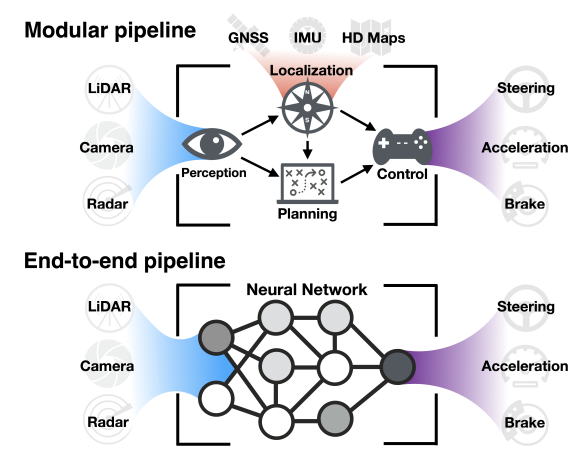
\includegraphics[width=0.4\linewidth, height=3.2cm]{images/end-modular.png} 
\label{fig:subim1}
%\end{subfigure}

\caption{Modular and end-end pipelines for autonomous driving\footcite{DBLP:journals/corr/abs-2003-06404}}
\label{fig:image2}
\end{figure}
\end{frame}

%--- Next Frame ---%
\begin{frame}{Motivation (2/5)}
  \textbf{Multi-task Learning vs Auxiliary Learning}

  \begin{itemize}
      \item By definition, both multi-task learning and auxiliary learning is the same. 
      \item In both cases we learn for multiple tasks by the sharing the same feature representation.
      \item The difference is that in auxiliary learning we give importance to the main task while utilizing the training signals from the correlated auxiliary tasks. 
  \end{itemize}
   
\end{frame}
%--- Next Frame ---%
\begin{frame}{Motivation (3/4)}
  \textbf{Multi-task Learning in Autonomous Driving}
  \begin{figure}[H]
     \centering
     
%\begin{subfigure}{\textwidth}
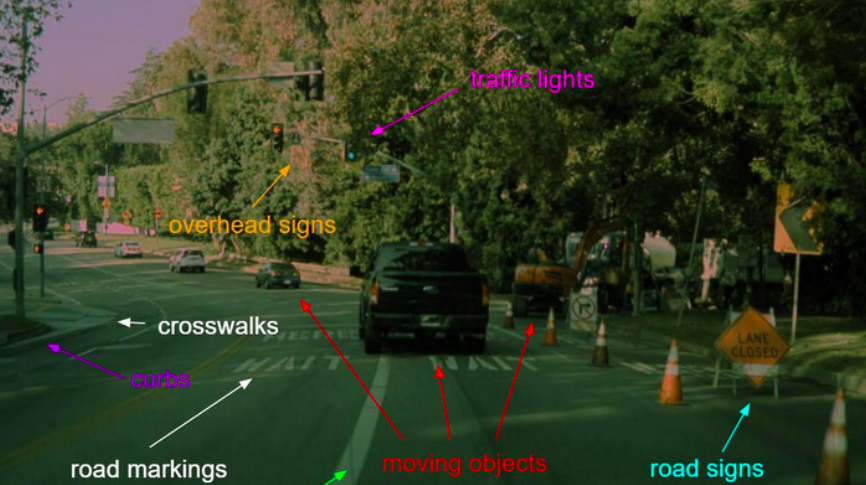
\includegraphics[width=0.6\linewidth, height=4.5cm]{images/MTL_aux.png} 
\label{fig:subim1}
%\end{subfigure}

\caption{Tasks to learn in a scene \footcite{tesla} }
\label{fig:image2}
\end{figure}
\end{frame}

%--- Next Frame ---%

   
\begin{frame}{Motivation (4/4)}
  \textbf{Challenges in Multi-task Learning for End-to-End Autonomous Driving
}

  \begin{itemize}
      \item Causal confusion
      \item Distribution shift 
      \item Selection of auxiliary tasks
      \item Simulation can not cover all the scenarios 
      \item Selection of a unified feature extractor 
      \item Task loss balancing
  \end{itemize}
\end{frame}

% %--- Next Frame ---%
% \begin{frame}{Motivation (5/5)}
% \textbf{Multi-task Learning in Autonomous Driving}
%    \begin{itemize}
%         \item In a driving scenario for an autonomous car to make decision we need to learn for tasks like road sign, moving objects, traffic lights and more.
%         \item Generally these auxiliary tasks are correlated with the main task of prediction of driving commands.
%        \item Thus learning for auxiliary tasks  along with the main task makes the driving driving policy more robust and interpret-able.
%        \item Multi-task learning is an important component of the end-to-end autonomous driving.
%    \end{itemize}
% \end{frame}

\begin{frame}{Lane Detection in Autonomous Driving}
    \begin{itemize}
        \item In this work we have used 3D Lane detection as an auxiliary task along with the prediction of the driving commands.
    \end{itemize}
    
    \textbf{Monocular 2D Lane Detection}
    \begin{itemize}
        \item Takes an RGB image from a front facing camera mounted on autonomous vehicle and provides the set of pixels which represents lane lines. 
        \item Both input and output are represented in the image space ie. why these approaches are called 2D
        % \item The basic assumption is that the ground plane is flat.
        
    \end{itemize}
    
    \textbf{Monocular 3D Lane Detection}
    \begin{itemize}
        \item In the driving scenarios where the roads are with different allevation.
        \item We need to obtain 3D points of the lanes to perform accurate motion planning.
        \item Provides real world 3D coordinates of the lane lines with respect to a camera coordinate system.
    \end{itemize}
\end{frame}
%%%%%%%%%%%%%%%%%%%
\begin{frame}{3D Lane Geometry}
    \begin{figure}[H]
     \centering
     
%\begin{subfigure}{\textwidth}
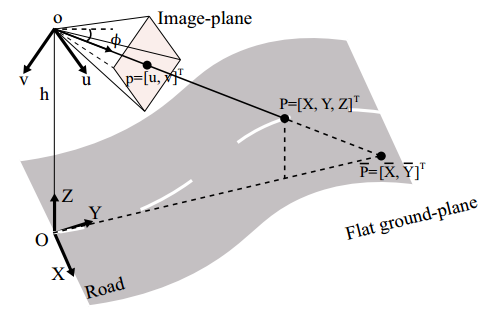
\includegraphics[width=0.6\linewidth, height=4cm]{images/3d_lane_geometry.png} 
\label{fig:subim1}
%\end{subfigure}

\caption{Geometric representation of lane point in 3D world space, image plane and virtual top view \footcite{DBLP:journals/corr/abs-2112-15351} }
\label{fig:image2}
\end{figure}
\end{frame}
% ----- next frame ------%
\begin{frame}{Inspiration for Proposed 3D Lane Detector (1/2)}
\textbf{Approach 1: Gen-LaneNet}

 \begin{figure}[H]
     \centering
     
%\begin{subfigure}{\textwidth}
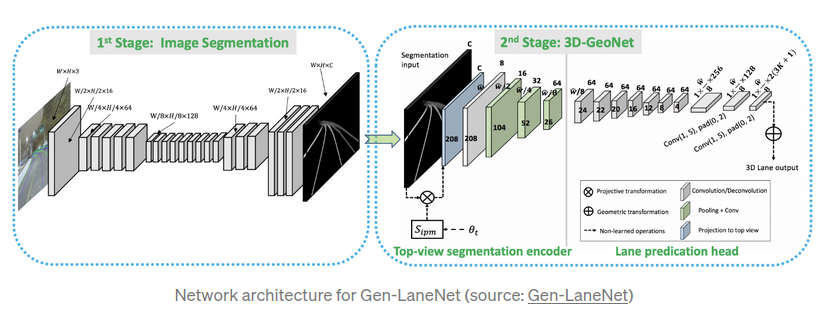
\includegraphics[width=0.8\linewidth, height=4cm]{images/genLanenet.png} 
\label{fig:subim1}
%\end{subfigure}

\caption{Gen-LaneNet pipeline \footcite{guo2020gen} }
\label{fig:image2}
\end{figure}
\end{frame}

%%%%%%%%%%%%%%%%%%%%%%%%%%

\begin{frame}{Inspiration for Proposed 3D Lane Detector (2/2)}
\textbf{Approach 2: Semi-local 3D-LaneNet}

 \begin{figure}[H]
     \centering
     
%\begin{subfigure}{\textwidth}
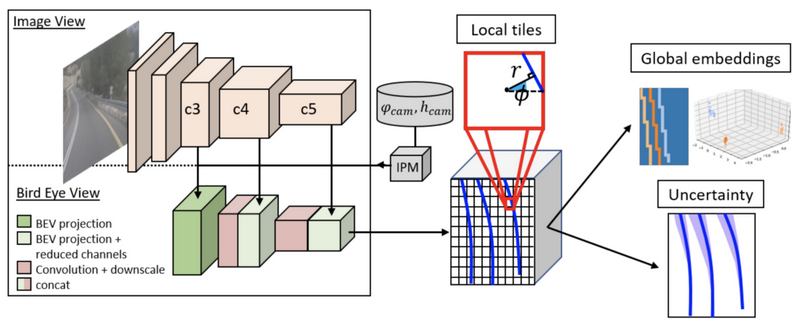
\includegraphics[width=0.8\linewidth, height=4cm]{images/3DLaneNET++.png} 
\label{fig:subim1}
%\end{subfigure}

\caption{Semi-local 3D LaneNet pipeline \footcite{DBLP:journals/corr/abs-2011-01535} }
\label{fig:image2}
\end{figure}
\end{frame}
%%%%%%%%%%%%%%%%%%%%%%%%%%%%%%%%
\begin{frame}{Pros and Cons of Previous Work (1/2)}
    \textbf{Gen-LaneNet}
    
    \begin{itemize}
        \item Dual stage pipeline is flexible in terms of replacing the first stage by better 2D lane detection algorithms. 
        \item Lane detection and prediction of 3D geometry are treated as different tasks. 
        % \item Introduced a generalized virtual top view for the correction of points in top view when a ego vehicle moves uphill or downhill.
        \item Can not handle different topologies when the lane lines are perpendicular to the ego vehicle.
        \item Can not generalize well with different cameras.
    \end{itemize}

\end{frame}

%%%%%%%%%%%%%%%%%%%%%%%%%
\begin{frame}{Pros and Cons of Previous Work (2/2)}
    \textbf{Semi-local 3D LaneNet}
    \begin{itemize}
        \item Prediction of 3D lane lines are done semi-locally and in an anchor-less manner. 
        \item Can generalize well to different topologies.
    \end{itemize}


\textbf{Takeaway}
\begin{itemize}
    \item We combine the effectiveness of dual stage pipeline proposed by Gen-LaneNet and semi-local anchor-less representation of the 3D lane curves  
\end{itemize}
\end{frame}

%%%%%%%%%%%%%%%%%%%%%%%%%%%
\begin{frame}{Proposed Dual Stage Semi-local Anchor-less 3D Lane Detector}


 \begin{figure}[H]
     \centering
     
%\begin{subfigure}{\textwidth}
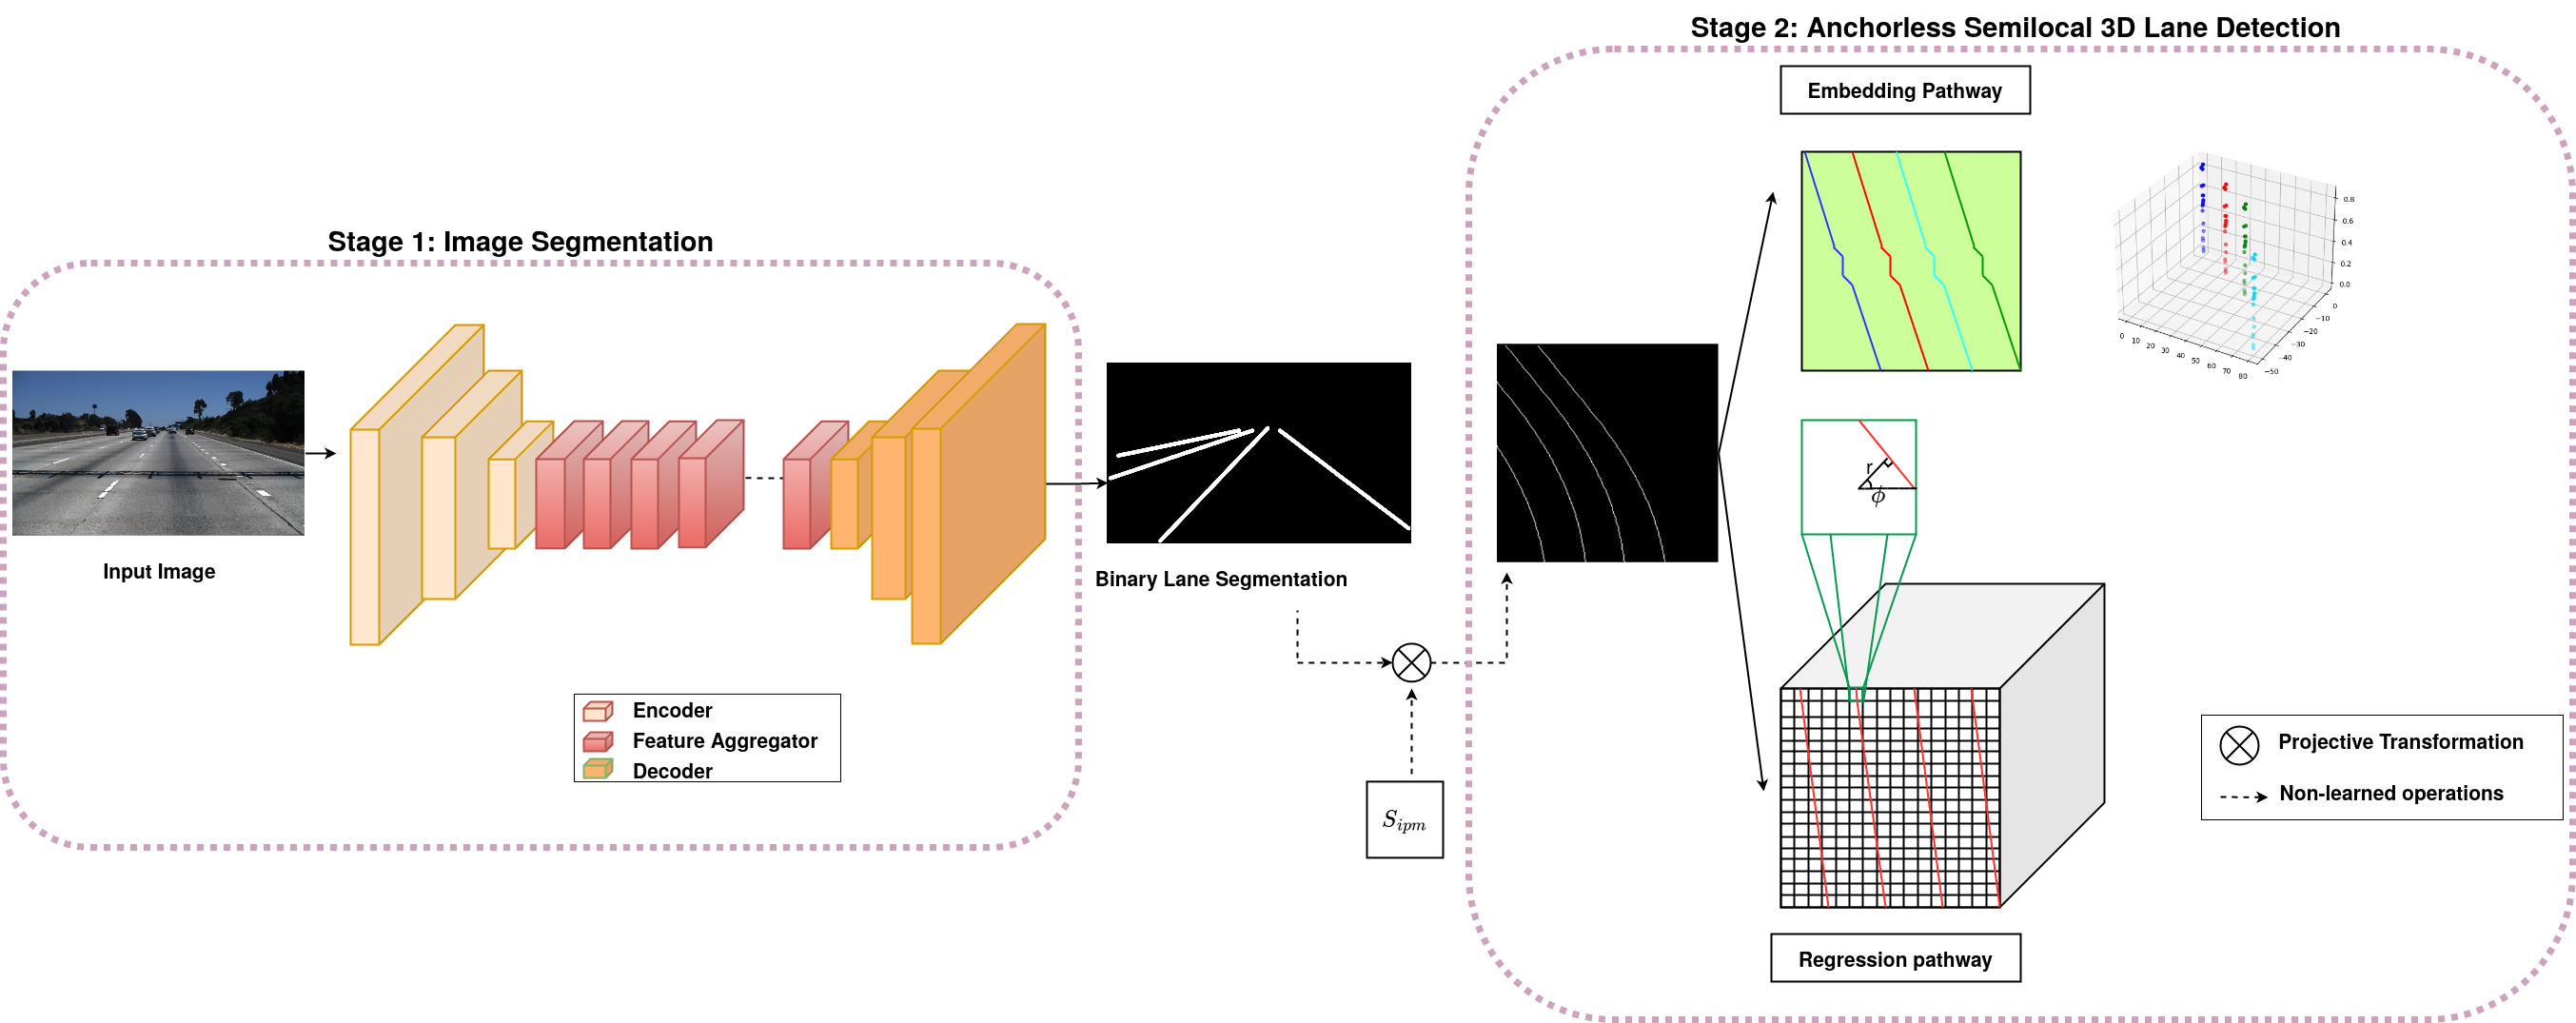
\includegraphics[width=0.8\linewidth, height=4.5cm]{images/3DlaneAUXNet.png} 
\label{fig:subim1}
%\end{subfigure}

\caption{Dual stage semi-local anchor-less 3D lane detection pipeline }
\label{fig:image2}
\end{figure}
\end{frame}

%%%%%%%%%%%%%%%%%%%%%%%%%%%%%%%%%%%%
%% Stage 1: Binary Lane Segmentation
%% s-1 DIAG... of pipeline 
%% s-2 mention why increased efficated RESNET ---- >  SCNN, RESA ---> decoders
%% s-3 Traning details and datasets used
%% s-4 Training Targets and Loss functions used
%% s-5 QA and EMP Results with cross entropy
%% s-6 QA and EMP Results after task loss balancing 
%% s-7 QA and EMP Results with combined GenLaneNet 

\begin{frame}{Stage 1: Binary Lane Segmentation}
    \begin{itemize}
        \item Subtask of 2D lane segmentation
        \item Instead of predicting multiple labels for different lanes, we obtain binary masks for the lane lines in the image.
    \end{itemize}

\begin{figure}[H]
     \centering
     
%\begin{subfigure}{\textwidth}
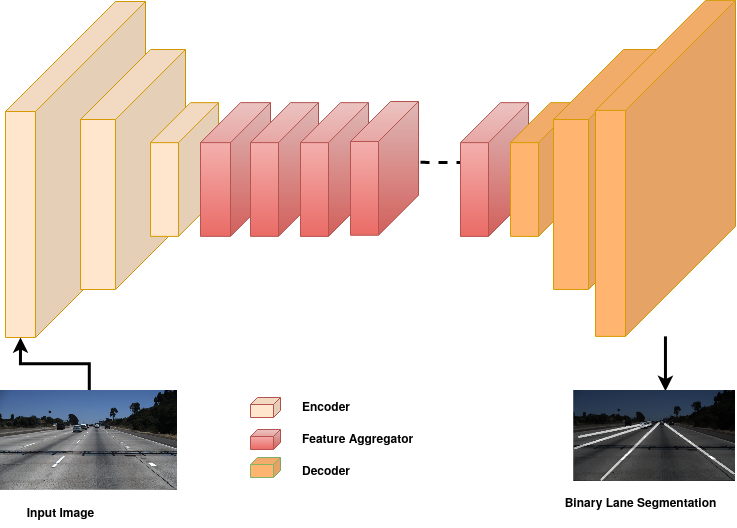
\includegraphics[width=0.4\linewidth, height=3cm]{images/2dlane_pipleline.png} 
\label{fig:subim1}
%\end{subfigure}

\caption{2D Binary Lane segmentation Pipeline \footcite{Tusimple} }
\label{fig:image2}
\end{figure}
\end{frame}
%%%%%%%%%%%%%%%%%%%%%

\begin{frame}{Selection of Network Architecture for Binary Lane Segmentation (1/2)}
    \textbf{Encoder}
    \begin{itemize}
        \item ResNet18 and ResNet50\footcite{DBLP:journals/corr/HeZRS15} are used as the main feature extractor.
        \item Dilated convolutions are used in the last layers of the feature extractor to increase the receptive field.
    \end{itemize}

    \textbf{Feature Aggregator}
    \begin{itemize}
        \item Features aggregator modules proposed by SCNN\footcite{pan2018SCNN} and RESA\footcite{DBLP:journals/corr/abs-2008-13719} are utilized.
        \item Both feature extractor are tailored for 2D lane segmentation.
    \end{itemize}
\end{frame}

\begin{frame}{Selection of Network Architecture for Binary Lane Segmentation (2/2)}
    \textbf{Decoder}
    \begin{itemize}
        \item Simple decoder proposed by SCNN, which used bi-linear interpolation to upsample the feature maps.
        \item Bilateral upsampling decoder (BUSD) propsed by RESA.
    \end{itemize}


    2D binary lane segmentation is trained via mix and match of the above mentioned encoder, decoder and feature aggregator modules.

\end{frame}
%%%%%%%%%%%%%%%%%%%%%%5

\begin{frame}{Loss Computation for 2D Binary Lane Segmentation}
    \begin{figure}[H]
     \centering
     
%\begin{subfigure}{\textwidth}
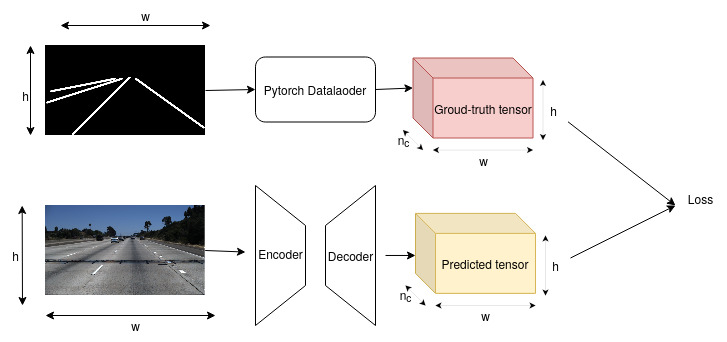
\includegraphics[width=0.6\linewidth, height=4cm]{images/2d_dataflow_loss_computation.jpg} 
\label{fig:subim1}
%\end{subfigure}

\caption{ Data flow for loss computation for 2D binary lane segmentation pipeline. w and h represents
the spatial size of the image tensors and $n_{c}$ represents the number of classes\footcite{Tusimple}}
\label{fig:image2}
\end{figure}
\end{frame}
%%%%%%%%%%%%%%%%%%%%%%%%%%%%%%%%%%%%%
\begin{frame}{Loss Functions: 2D Binary Lane Segmentation}
    \textbf{Cross Entropy Loss}
    \begin{equation}
        L_{CCE} = -\frac{1}{N}\sum_{i=1}^{N} \sum^{M}_{j=1}y_{i,j}\cdot log(p_{i,j})
        \end{equation}
        where $p_{i,j}$ is the prediction for each class and $y_{i,j}$ is the target value for each class. N and M are the number of rows and columns.
    
    \textbf{Dice Loss}

    \begin{equation}
            DC = \frac{2TP}{2TP + FP + FN} = \frac{2|X \cap Y|}{|X| + |Y|}
        \end{equation}
    where $TP$ ,$FP$ and $FN$ are the true positives, false positives and false negatives.  
        
        \begin{equation}
            L_{dice} = 1 - DSC
        \end{equation}
    
\end{frame}
%%%%%%%%%%%%%%%%%%%%%%%%%%%%
\begin{frame}{Loss Functions: 2D Binary Lane Segmentation}

\textbf{Focal Loss}

\begin{equation}
            Cross Entropy = - \sum^{n}_{i=1}Y_{i}log(p_{i})
        \end{equation}
        where $Y$ and $p$ represents the is the ground-truth label and the predicted probability.
        
        \begin{equation}
            Focal Loss = - \sum^{i=n}_{i=1} \alpha_{i}(1-p_{i})^{\gamma} log_{b}(p_{i})
        \end{equation}
        
         when $\gamma = 0$, Focal Loss is equal to Cross Entropy Loss.
\end{frame}

\begin{frame}{Datasets Used}
    \begin{itemize}
        \item TuSimple\footcite{Tusimple} - simple dataset consists of normal highway driving.
        \item CULane\footcite{pan2018SCNN} - complex dataset consists urban driving scenarios with different weather conditions.
        \item Apollo Synthetic Dataset (Sim3D)\footcite{guo2020gen} - synthetic 3D lane detection dataset.
    \end{itemize}
\end{frame}

\begin{frame}{Evaluation Metric Used}
    
    \begin{itemize}
        \item IoU (Intersection-over-union) or Jaccard index is used to evaluate the trained models.
    \end{itemize}
    \begin{figure}[H]
     \centering
     
%\begin{subfigure}{\textwidth}
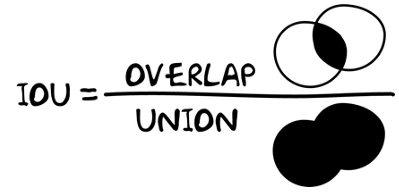
\includegraphics[width=0.5\linewidth, height=3cm]{images/IOU.png} 
\label{fig:subim1}
%\end{subfigure}

\caption{ (IoU)Intersection-Over-Union\footcite{IOU}}
\label{fig:image2}
\end{figure}
\end{frame}

%%%%%%%%%%%%%
\begin{frame}{Results for Binary Lane Segmentation: Cross Entropy Loss}
    \begin{itemize}
        \item Initially models are trained on CULane , TuSimple and Apollo Synthetic dataset (sim3D) with Cross Entropy loss as our objective function. 
    \end{itemize}

    \begin{table}[h!]
    \caption{Results for binary lane segmentation using Cross Entropy loss as the loss function}
    \centering
    \begin{tabular}{|l|l|l|}
    \hline
        \textbf{Method} & \textbf{IoU} & \textbf{FPS} \\ \hline
        SCNN(Res18+TuSimple) & 54.81 & $\approx$ \textbf{70}  \\ \hline
        RESA(Res18+TuSimple)  & 56.73 & $\approx$ 50 \\\hline
        SCNN(Res18+CUlane)  & 38.1 & $\approx$ 70 \\ \hline
        RESA(Res18+CUlane)& 43.23 &  $\approx$ 45\\\hline
        SCNN(Res18+sim3d) & 44.12 & $\approx$ 70 \\ \hline
        RESA(Res18+sim3d) & 71.79 & $\approx$ 45 \\ \hline
        RESA(Res50+sim3d) & \textbf{74.11} & $\approx$ 40 \\ \hline
        
    \end{tabular}
\end{table}
\end{frame}

%%%%%%%%%%%%%%%
\begin{frame}{Qualitative Results Binary Lane Segmentation: CE Loss}
\begin{columns}[t]
        \column{.5\textwidth}
        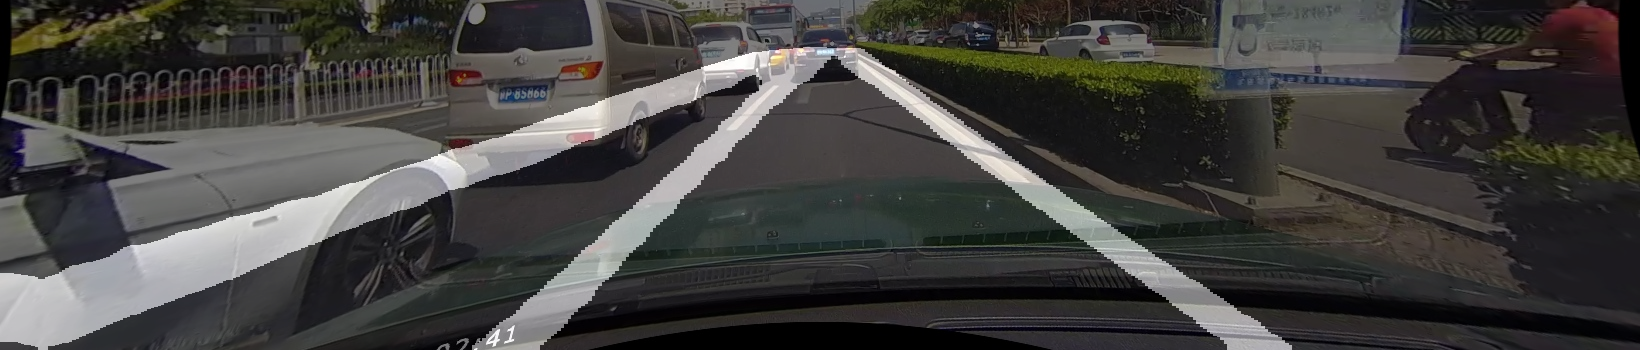
\includegraphics[width=\columnwidth,height= 2cm]{images/SCNN_res_culane.png}
        \centering
        \captionof{(a)}{SCNN (Res18+CULane) \footcite{pan2018SCNN}}
        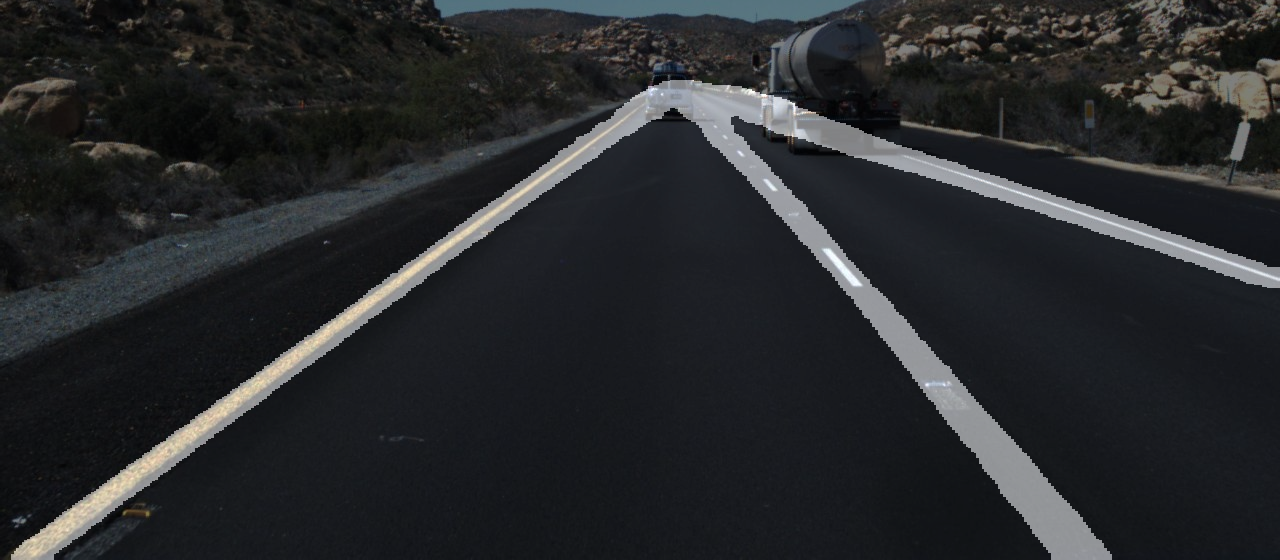
\includegraphics[width=\columnwidth,height= 2cm]{images/SCNN_res_tusimple.png}
        \captionof{(b)}{SCNN (Res18 + TuSimple) \footcite{Tusimple}}
        \column{.5\textwidth}
        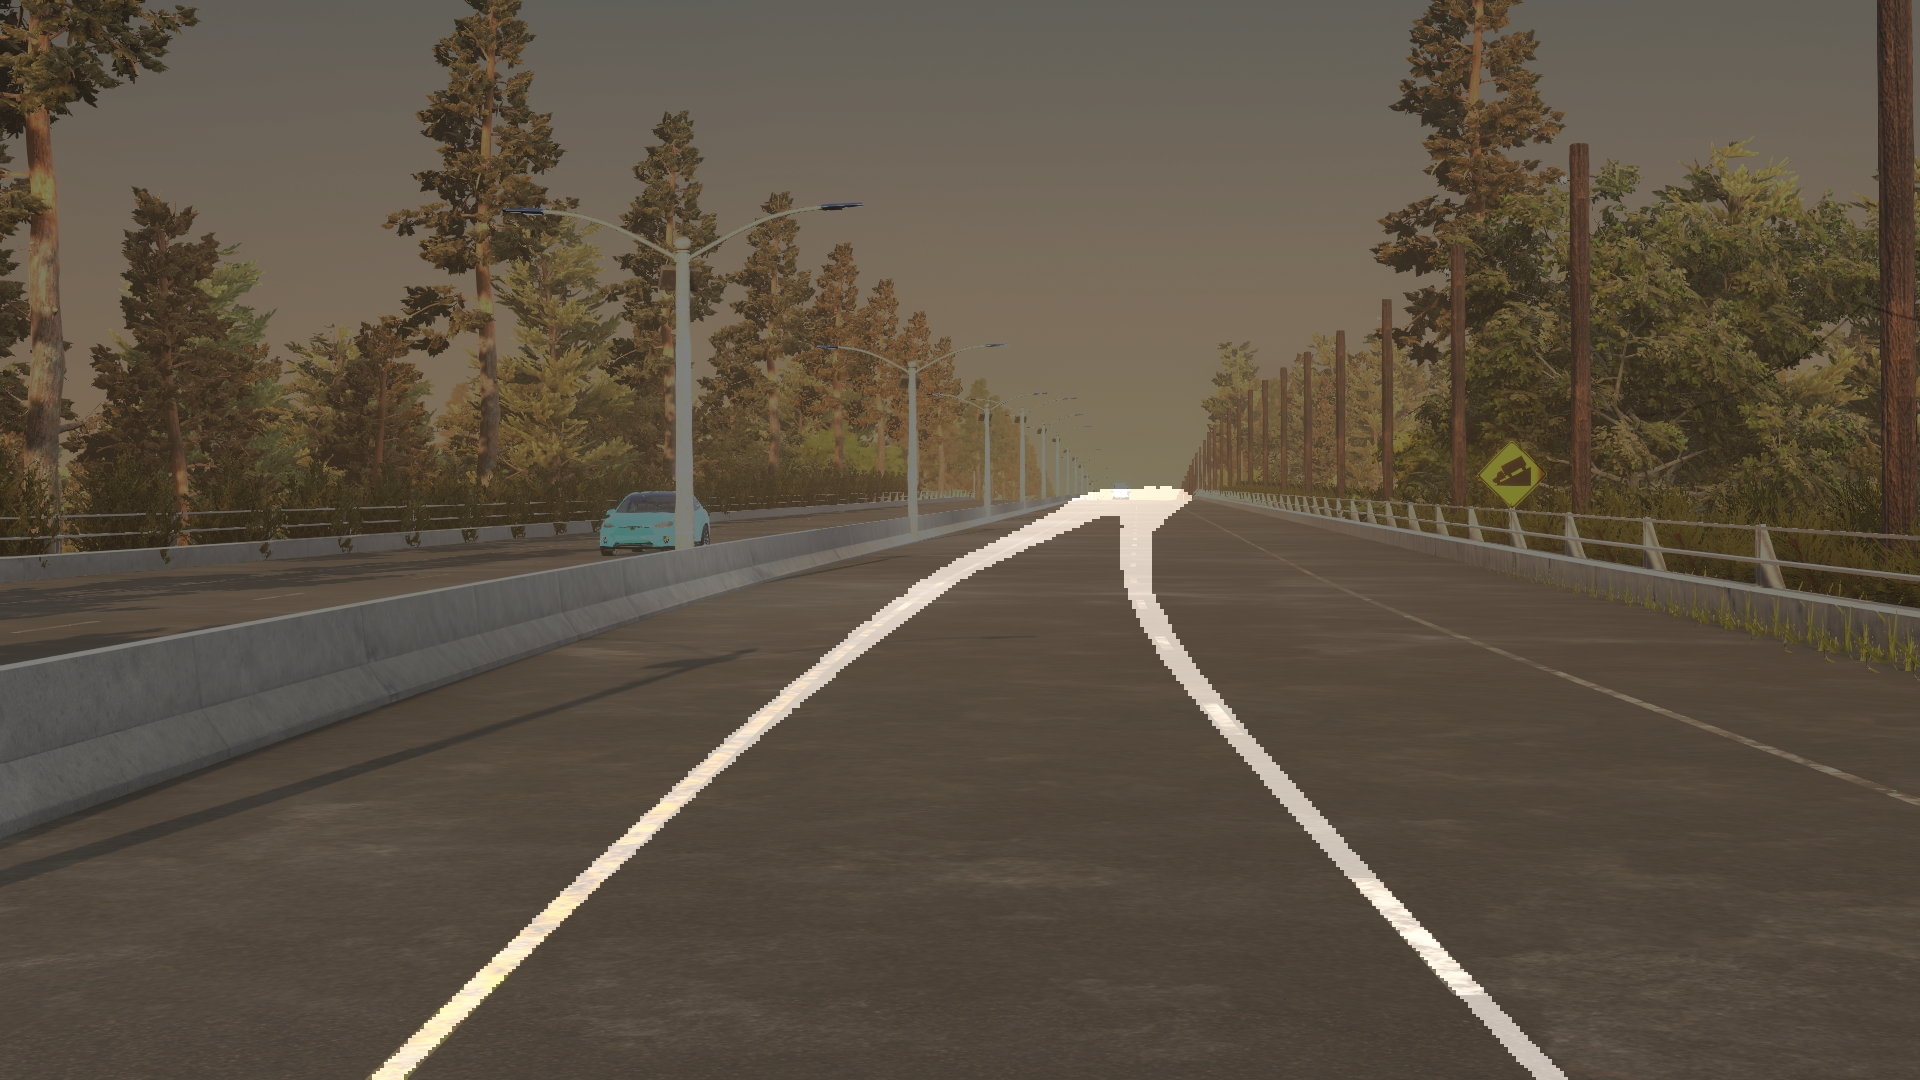
\includegraphics[width=\columnwidth,height= 2cm]{images/Resa_r18_sim3d.png}
        \centering
        \captionof{(c)}{RESA (Res18 + sim3d) \footcite{guo2020gen}}
    \end{columns}

\end{frame}


%%%%%%%%%%%%%%%%

\begin{frame}{Addressing the Class Imbalance Problem}
\begin{itemize}
    \item Number of pixels occupied by lanes are lesser than the background.
    \item Cross Entropy considers the loss globally not locally. 
    \item Occurrence of one class overpowered the other leads to class imbalance problem.
    \item To counter this, weighted CE Loss, focal and dice loss is used. 
\end{itemize}

    \begin{table}[h!]
    \caption{Quantitative results for binary lane segmentation trained on sim3d dataset using Cross Entropy Loss, Focal Loss and Dice Loss}
    \centering
    \begin{tabular}{|l|l|l|}
    \hline
        \textbf{Method} & \textbf{IoU} & \textbf{FPS} \\ \hline
        RESA(Res18+Cross Entropy)  & 71.79 & $\approx$ 45 \\ \hline
        SCNN(Res18+Cross Entropy) & 44.12 & $\approx$ \textbf{70}  \\ \hline
        RESA(Res50+Cross Entropy)  & 74.11 & $\approx$ 40  \\ \hline

        RESA(Res18+Dice Loss) & 82.57 & $\approx$ 50 \\\hline
        RESA(Res50+Dice Loss) & \textbf{83.33} & $\approx$ 50 \\\hline
    \end{tabular}
\end{table}
\end{frame}

%%%% Qulitative results for EGO vehicle with focal and dice loss on sim3d 
\begin{frame}{After Addressing The Class Imbalance Problem (1/4)}
\begin{columns}[t]
        \column{.5\textwidth}
        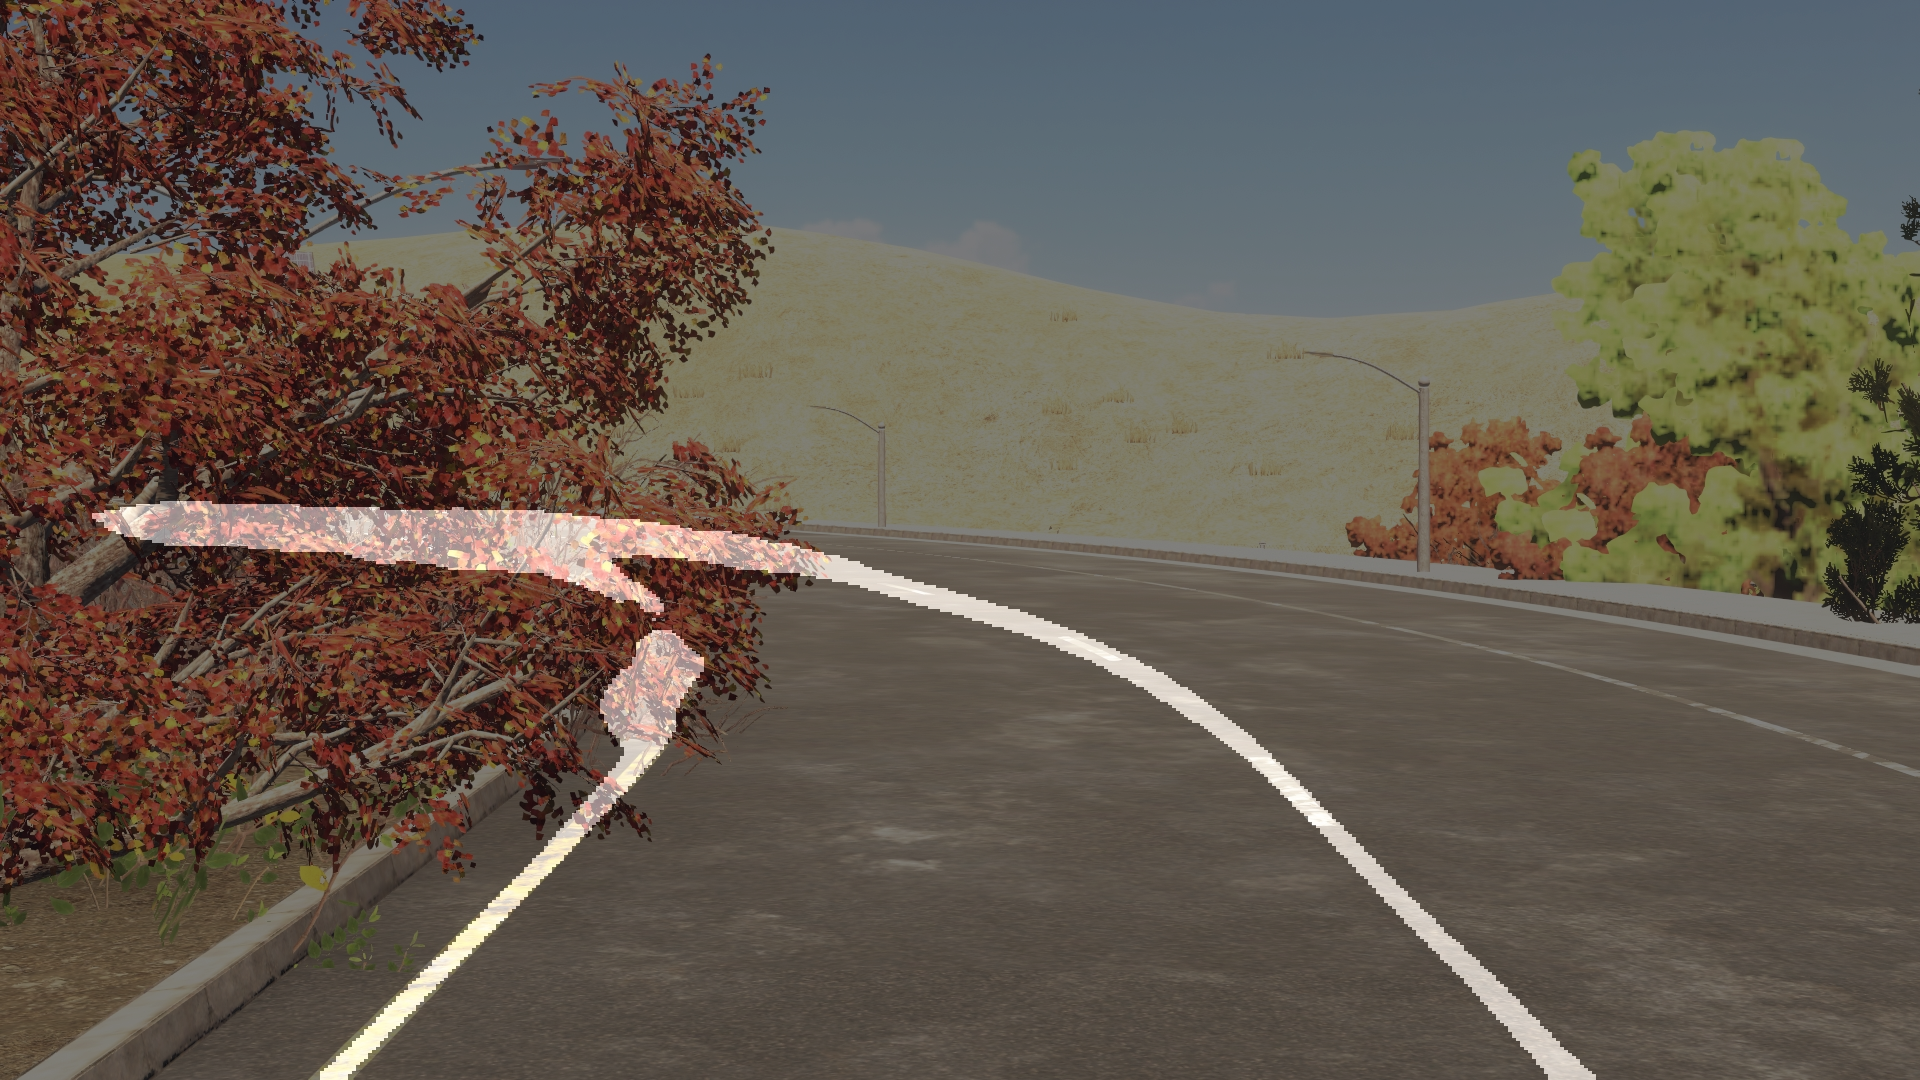
\includegraphics[width=\columnwidth,height= 2cm]{images/binseg_ce_resa.png}
        \centering
        \captionof{(a)}{ RESA(Res18+Cross Entropy Loss) }
        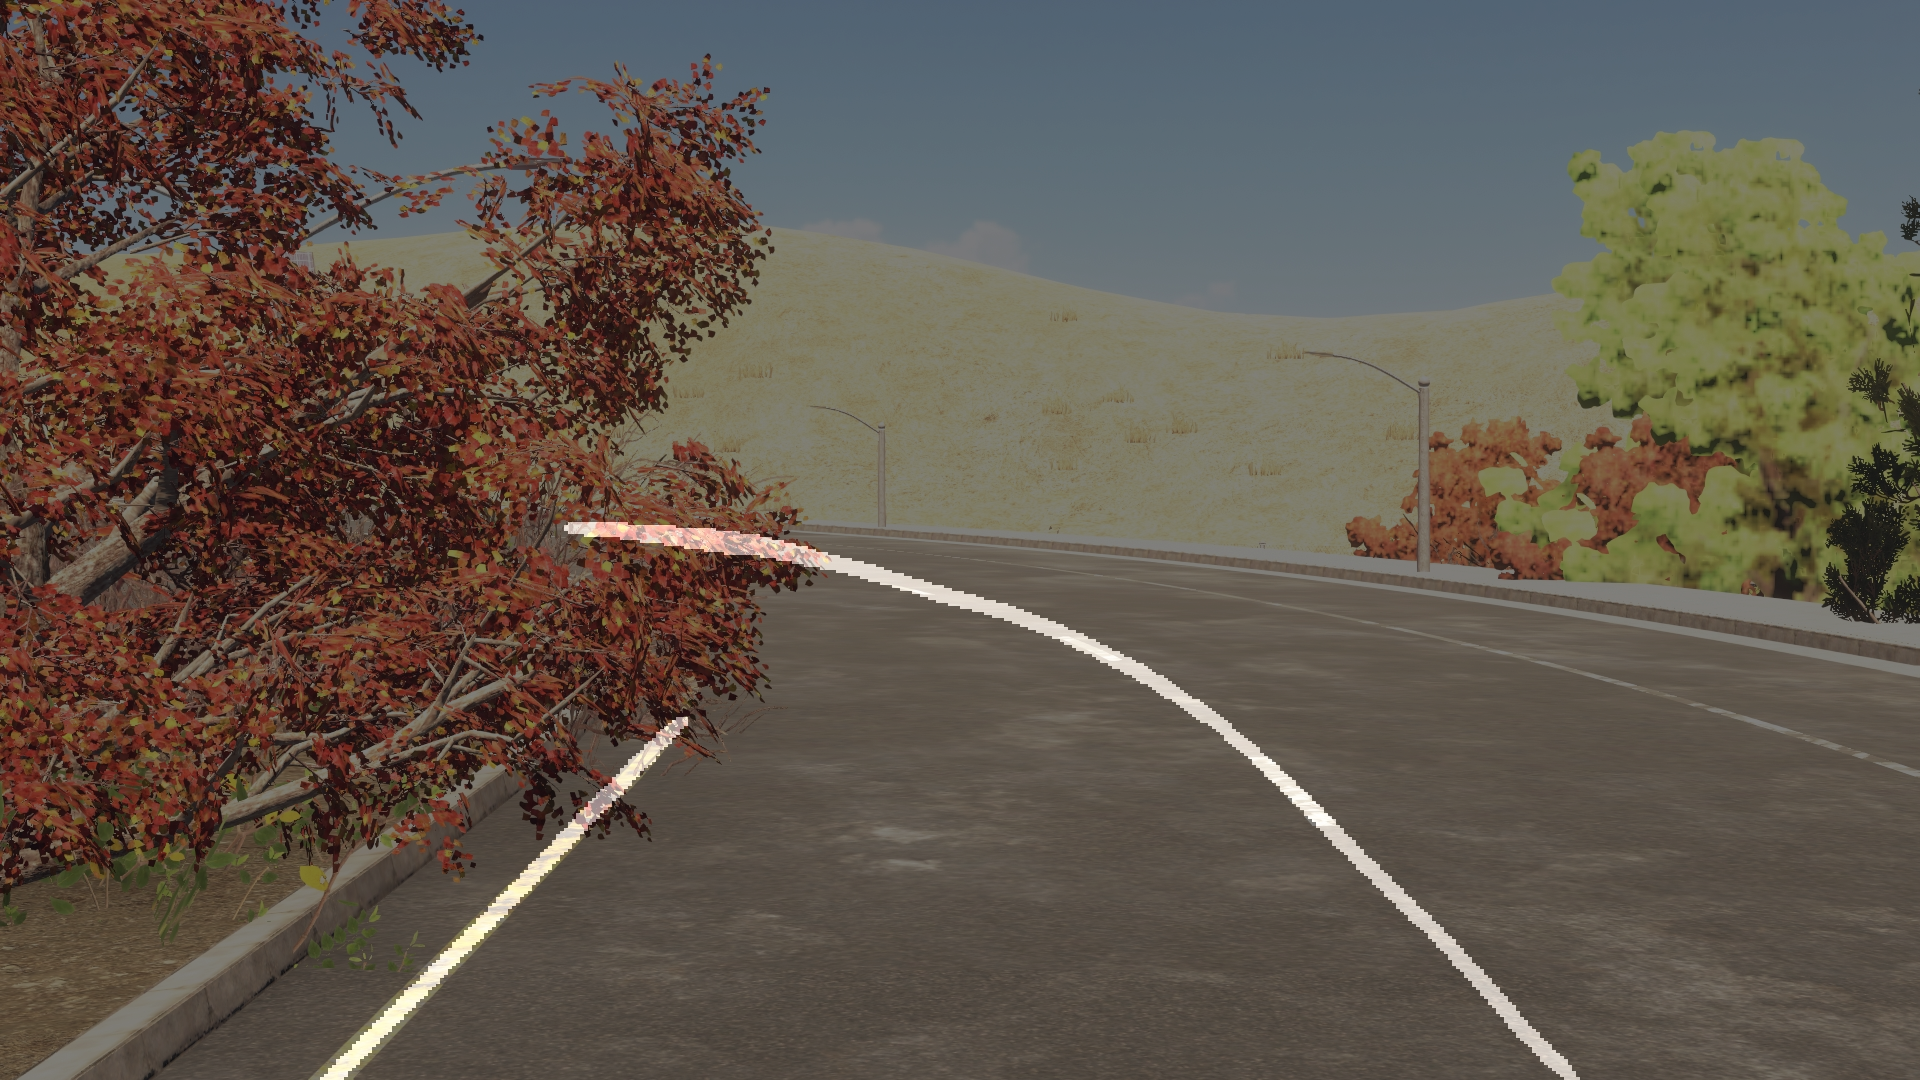
\includegraphics[width=\columnwidth,height= 2cm]{images/binseg_dice_resa.png}
        \captionof{(b)}{RESA(Res18+Dice Loss) }
        \column{.5\textwidth}
        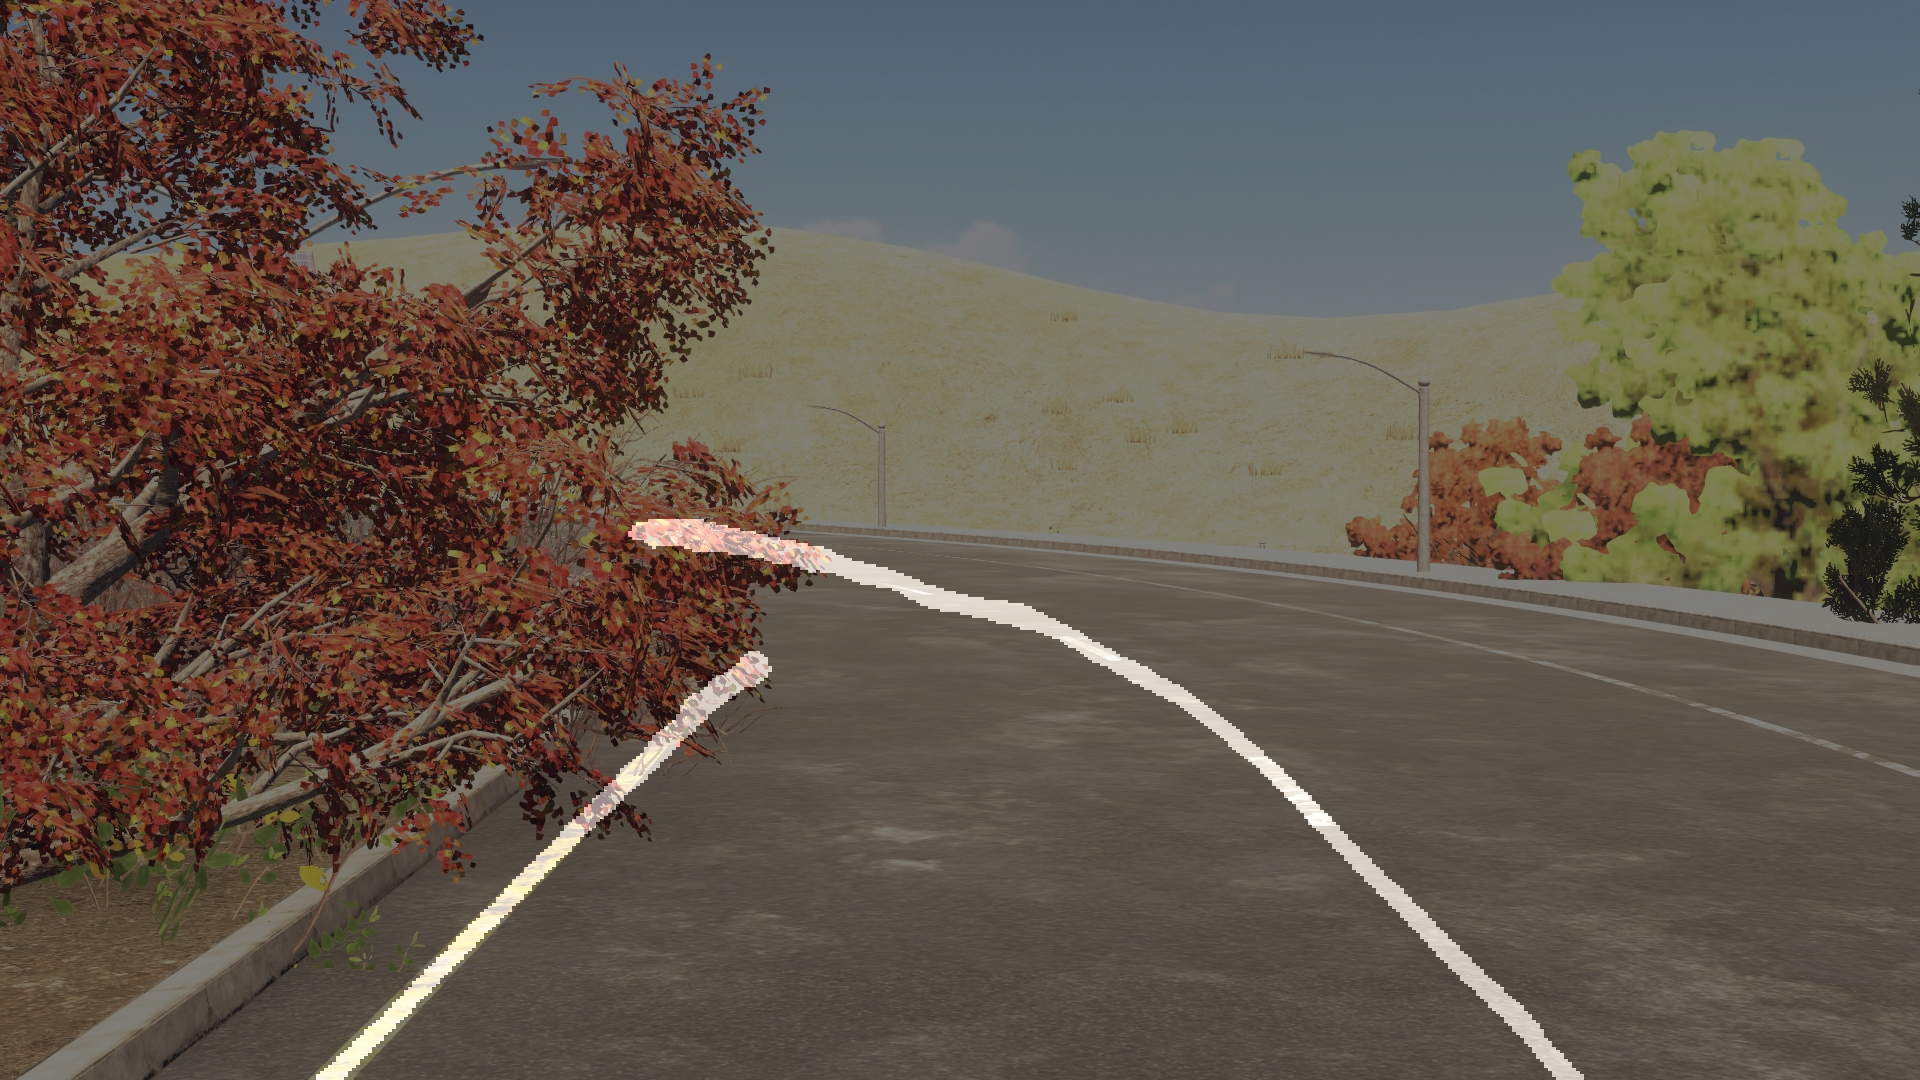
\includegraphics[width=\columnwidth,height= 2cm]{images/binseg_focal_resa.png}
        \centering
        \captionof{(c)}{ RESA(Res18+Focal Loss)\footcite{guo2020gen}}
    \end{columns}

\end{frame}
%%%%% Qualitative results for full lanes with focal and dice loss on sim3d
\begin{frame}{After Addressing The Class Imbalance Problem (2/4)}
\begin{columns}[t]
        \column{.5\textwidth}
        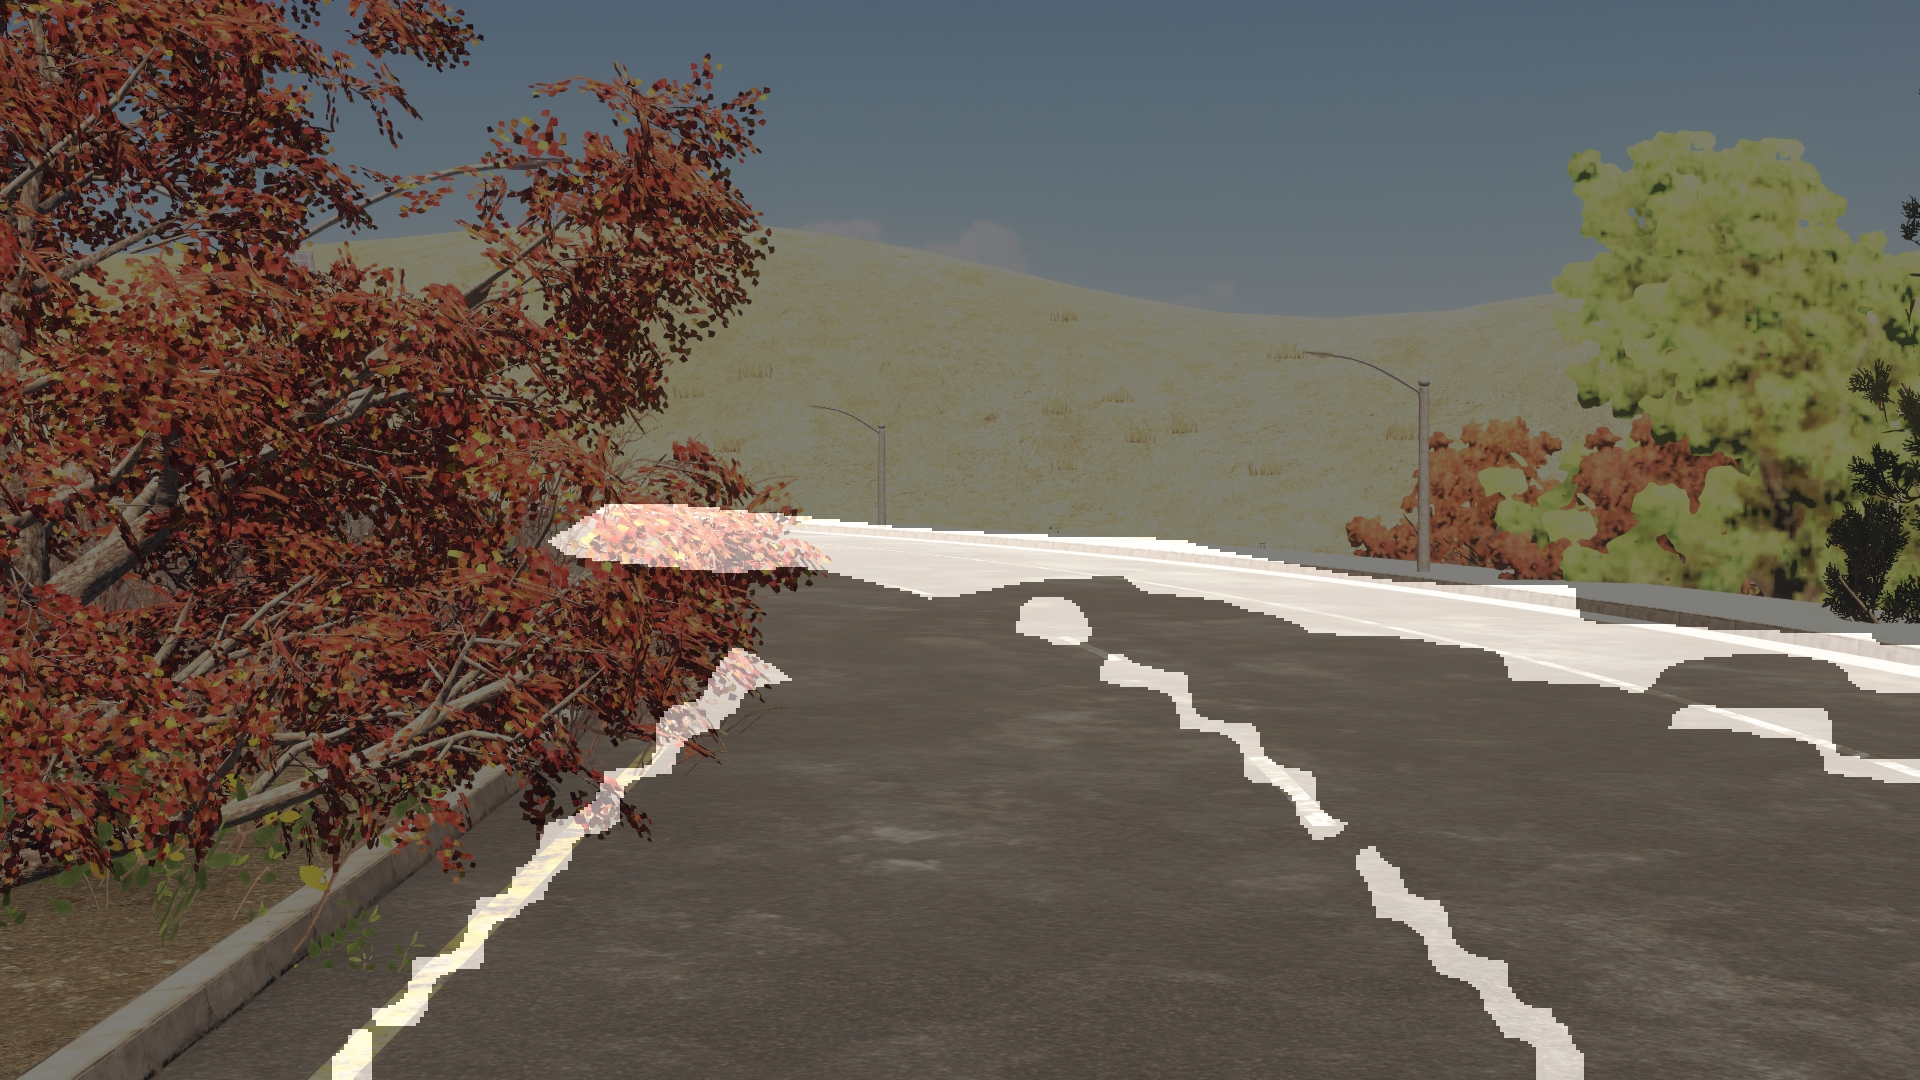
\includegraphics[width=\columnwidth,height= 2cm]{images/full_res18_scnn_focal.png}
        \centering
        \captionof{(a)}{ SCNN(Res18+Focal Loss)}
        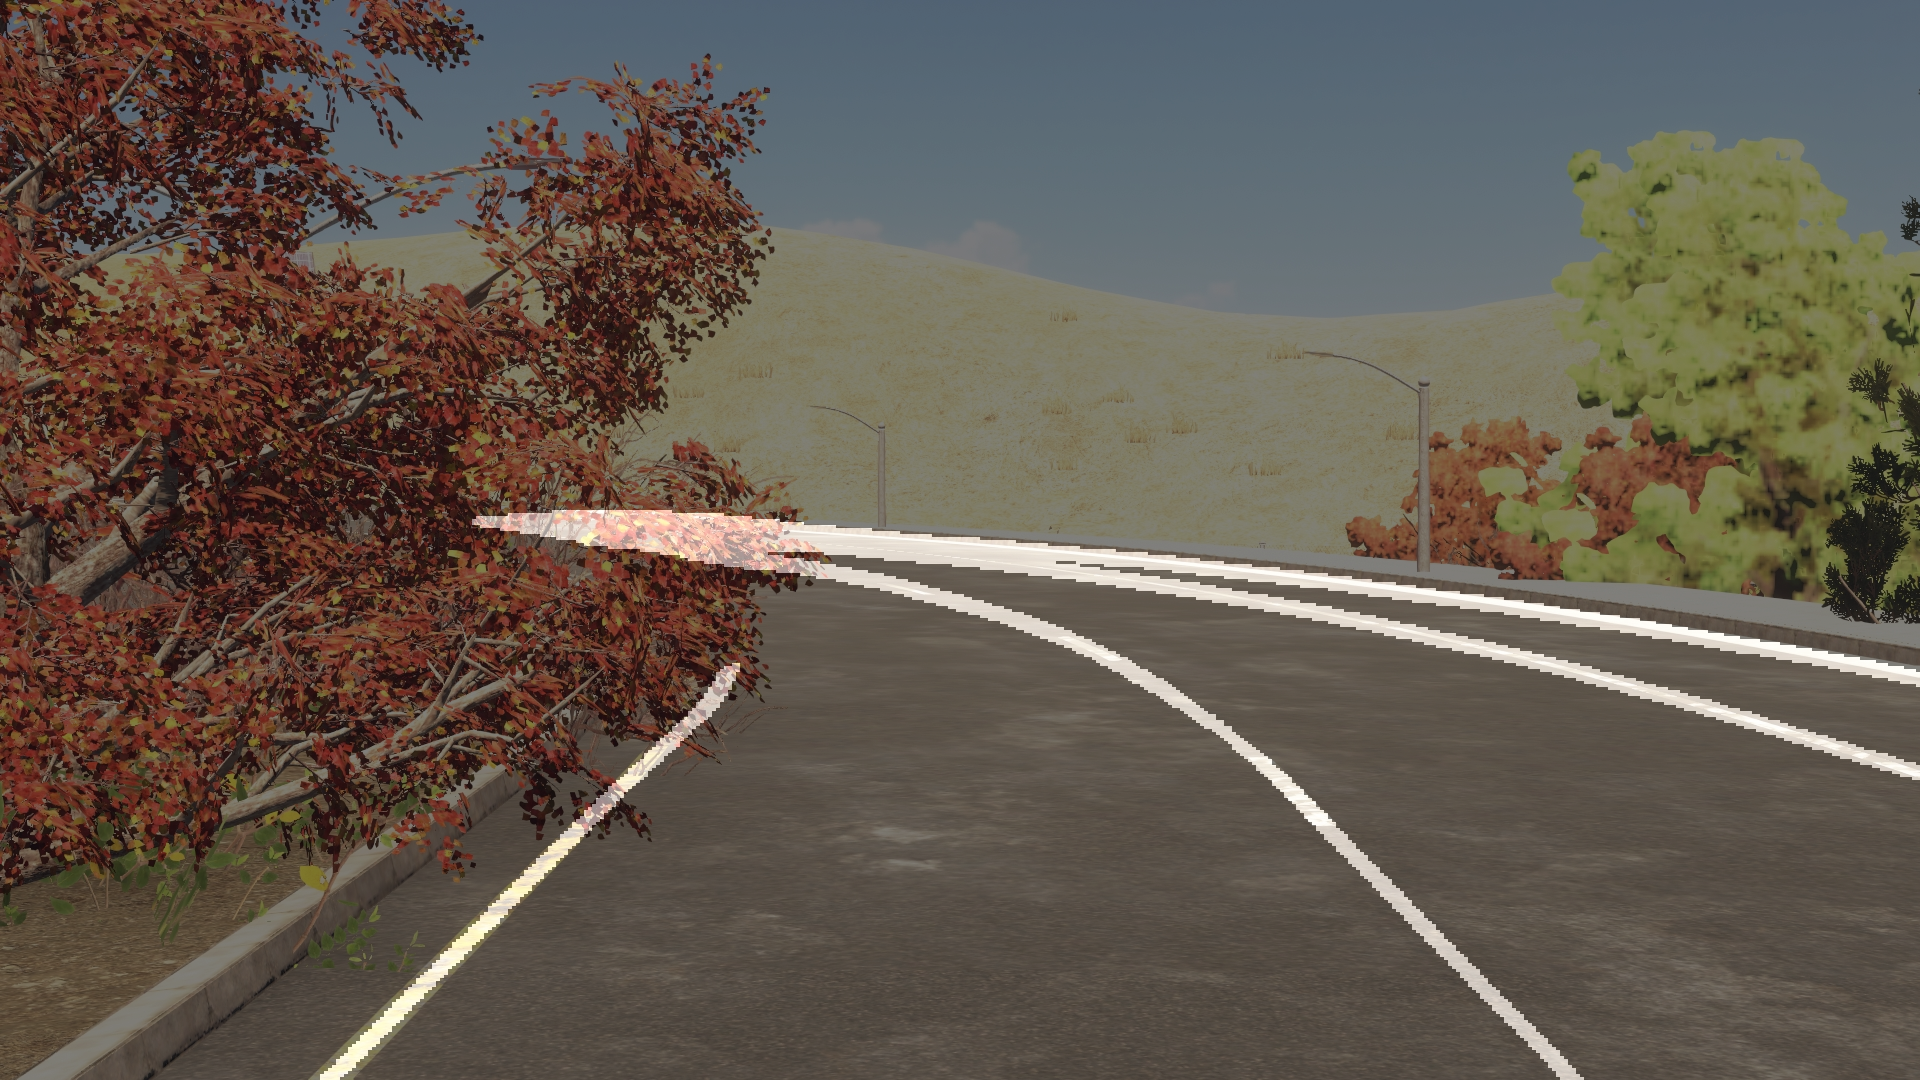
\includegraphics[width=\columnwidth,height= 2cm]{images/Resa_r18_full_dice.png}
        \captionof{(b)}{RESA(Res18+Dice Loss)}
        \column{.5\textwidth}
        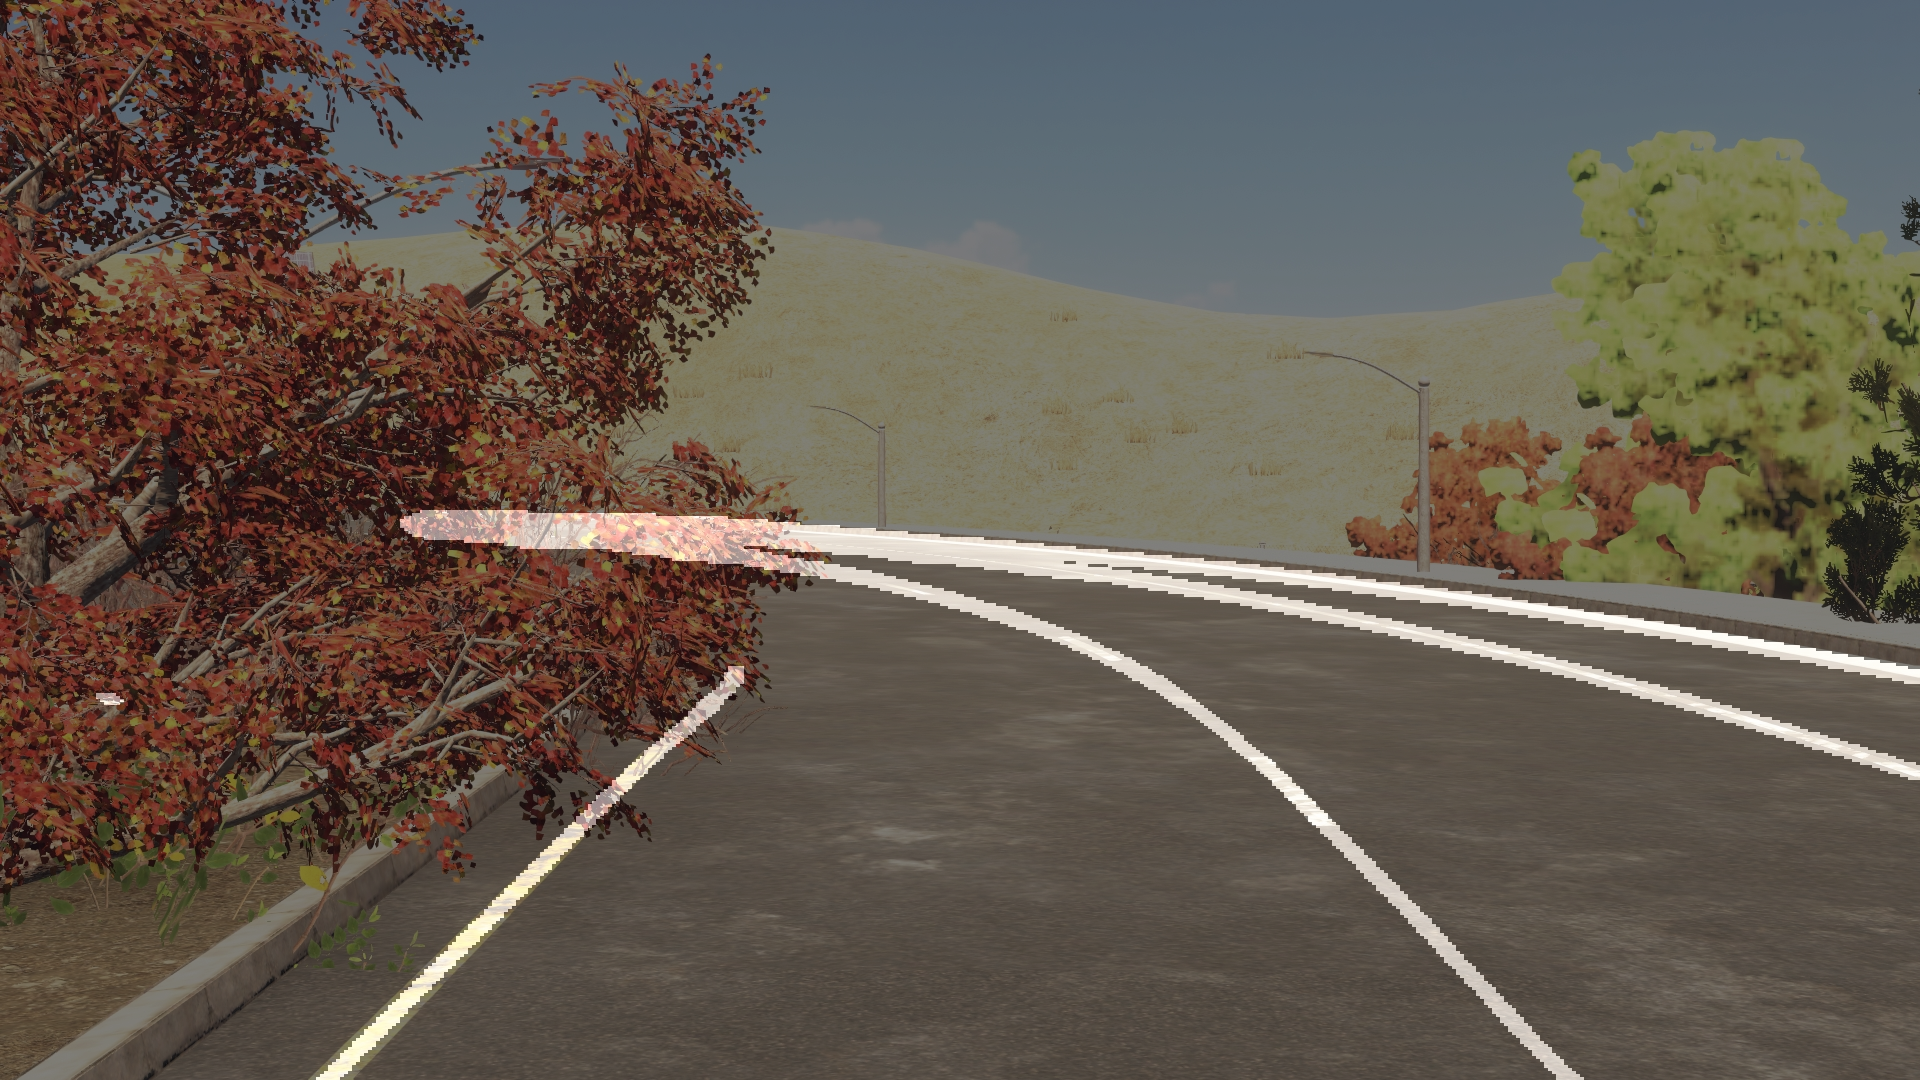
\includegraphics[width=\columnwidth,height= 2cm]{images/Resa_r50_full_dice.png}
        \centering
        \captionof{(c)}{ RESA(Res18+Focal Loss) \footcite{guo2020gen}}
    \end{columns}

\end{frame}

%%% Table 
\begin{frame}{After Addressing The Class Imbalance Problem (3/4)}
 \begin{table}[h]
    \caption{Quantitative results for binary lane segmentation on sim3D dataset for all the lanes present in the scene for all the lanes present in the scene.}
    \centering
    \begin{tabular}{|l|l|l|}
    \hline
        \textbf{Method} & \textbf{IoU} & \textbf{FPS} \\ \hline
        SCNN(Res18+Focal Loss)& 44.01 & $\approx$ \textbf{70} \\\hline
        RESA(Res18+Dice Loss) & 86.56 & $\approx$ 55 \\\hline
        RESA(Res50+Dice Loss) & \textbf{86.67} & $\approx$ 50 \\\hline
    \end{tabular}
\end{table}
    
\end{frame}
%%%% Compare the IOU curves 

\begin{frame}{After Addressing The Class Imbalance Problem (4/4)}

 % Iou curves for binary lane segmentation trained on sim3d dataset with CE loss, focal loss and dice loss for ego lane and all lanes.

% \begin{columns}[t]
%         \column{.5\textwidth}
%         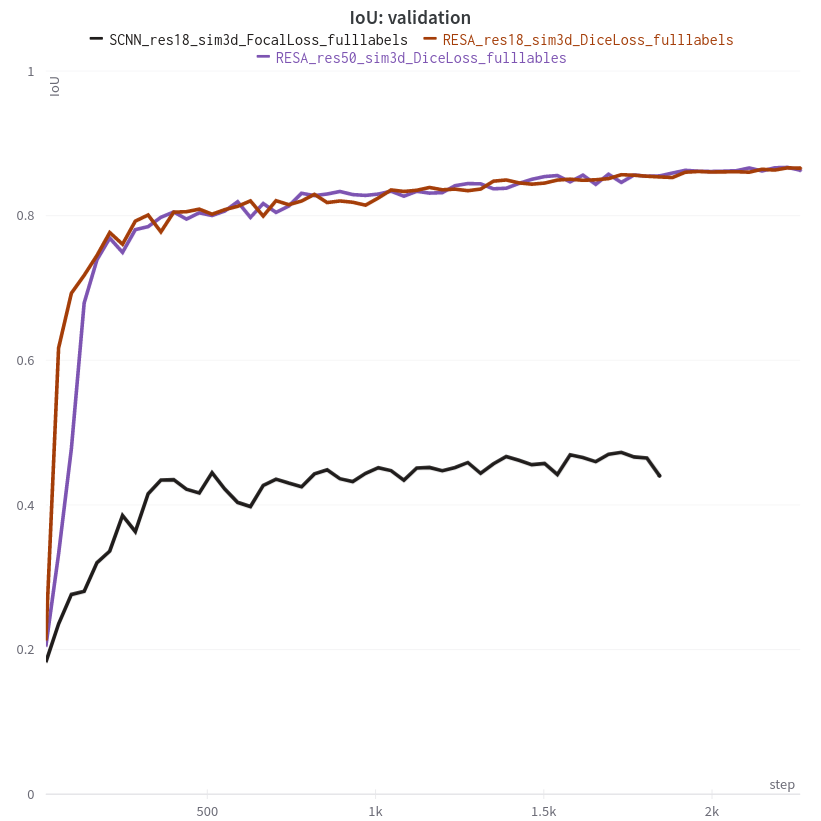
\includegraphics[width=0.5\columnwidth,height= 2cm]{images/change1.png}
%         \centering
%         \captionof{(a)}{ SCNN(Res18+Focal Loss)}
%         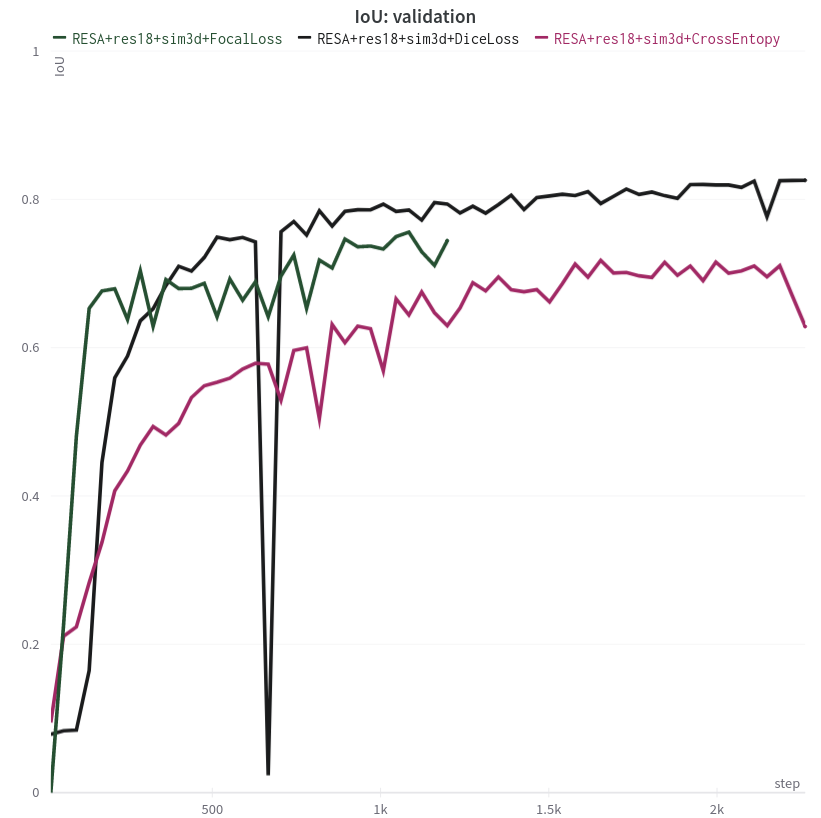
\includegraphics[width=0.5\columnwidth,height= 2cm]{images/change2.png}
%         \captionof{(b)}{RESA(Res18+Dice Loss)}
%         \column{.5\textwidth}
%     \end{columns}
% \begin{figure}[H]
%      \centering
     
% %\begin{subfigure}{\textwidth}
% 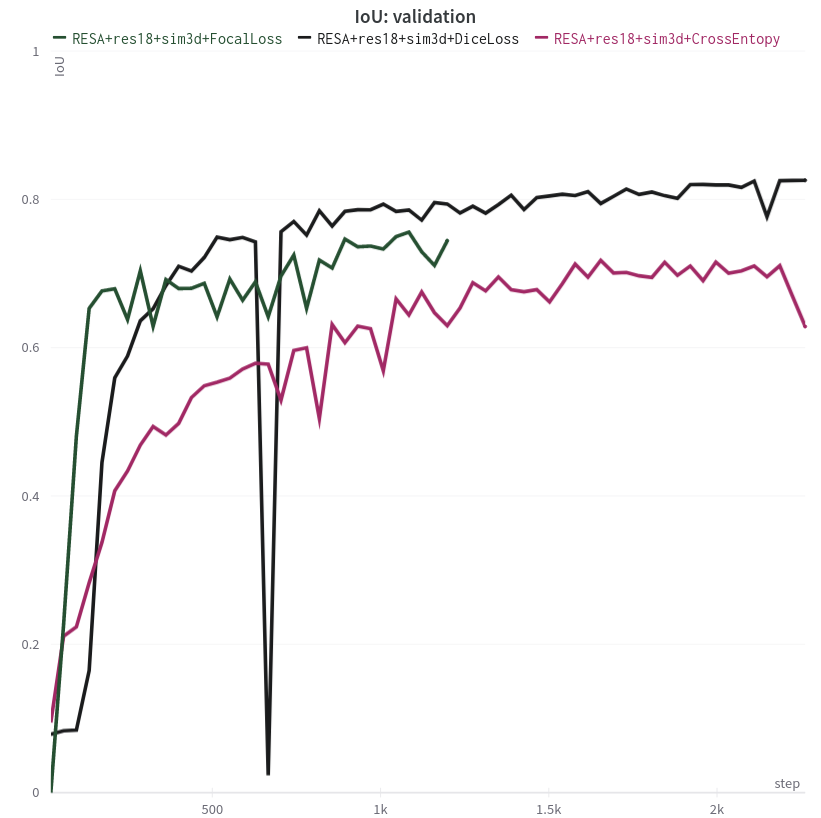
\includegraphics[width=0.4\linewidth, height=3cm]{images/change2.png} 
% \label{fig:subim1}
% %\end{subfigure}

% 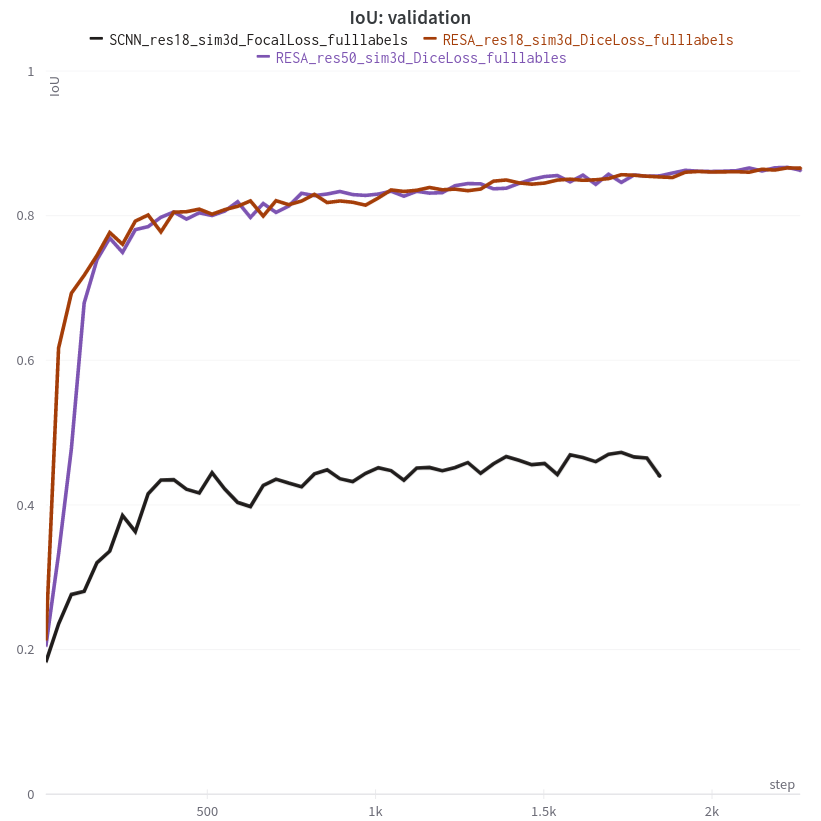
\includegraphics[width=0.4\linewidth, height=3cm]{images/change1.png} 
% \label{fig:subim1}
% \caption{ (IoU)Intersection-Over-Union}
% \label{fig:image2}
% \end{figure}

% \begin{columns}[t]
%     \column{.1\textwidth}
%         %\begin{center}
%             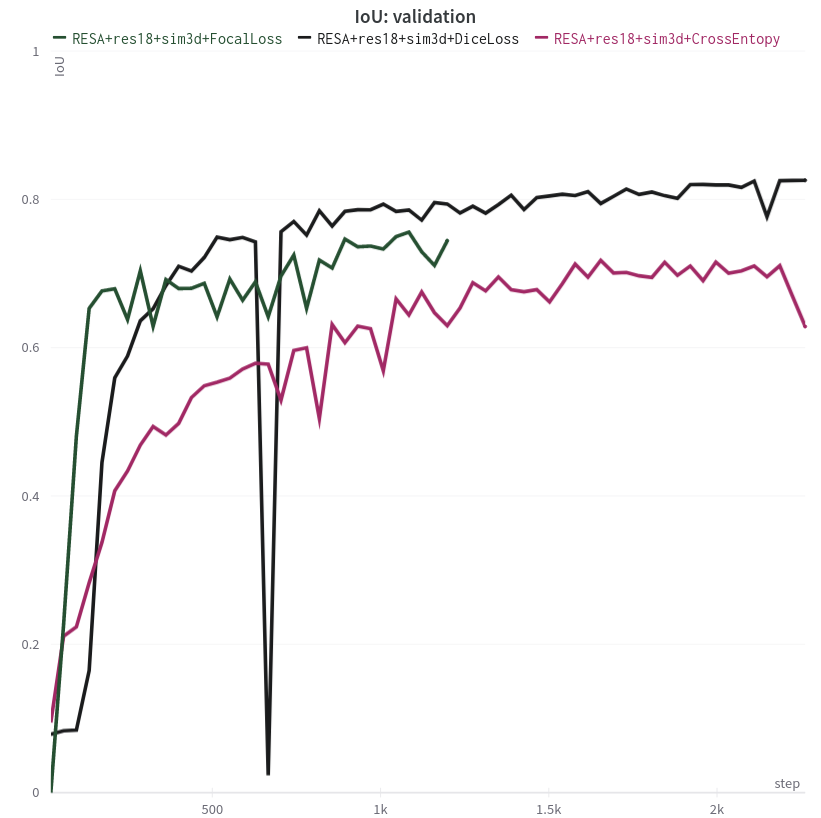
\includegraphics[scale=0.2]{images/change2.png}
%         %\end{center}
%     \column{.1\texwidth}
%         %\begin{center}
%              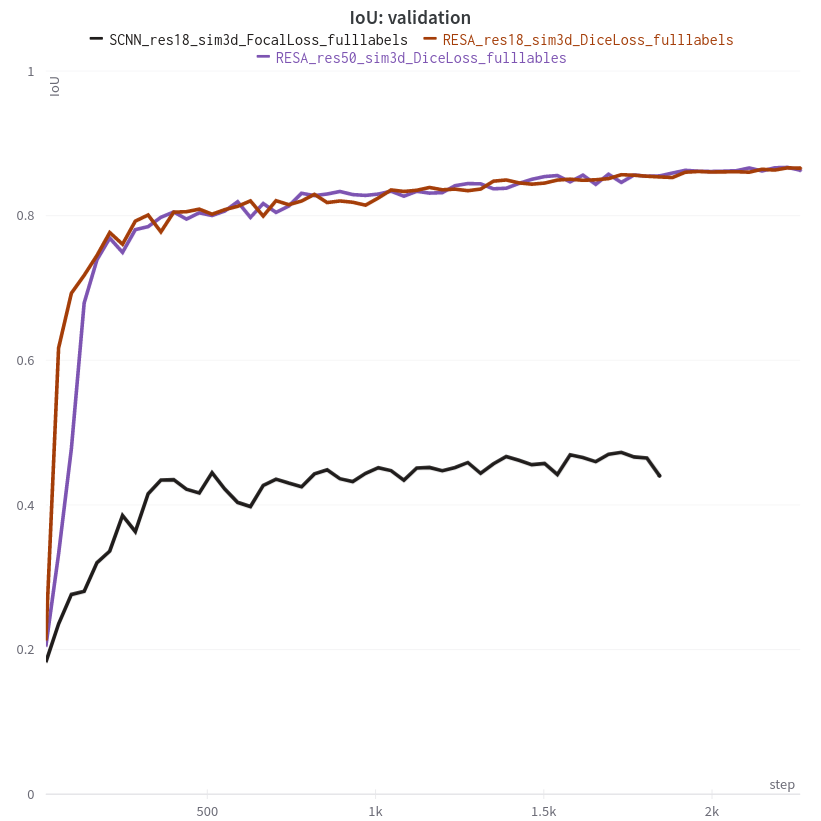
\includegraphics[scale=0.2]{images/change1.png} 
%         %\end{center}
% \end{columns}


\begin{figure}
   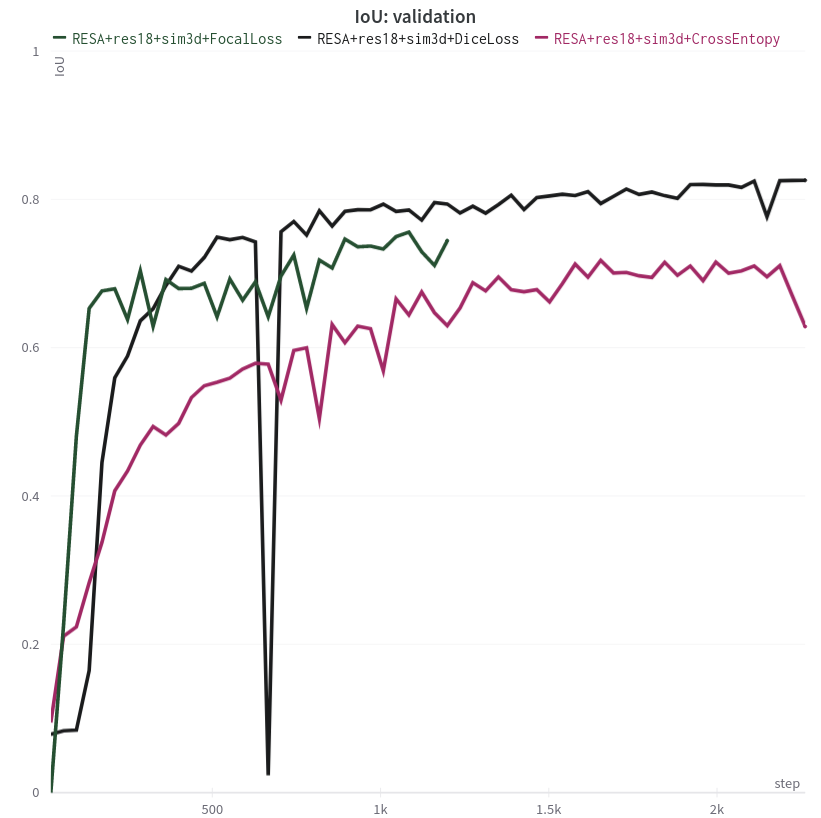
\includegraphics[scale=0.2]{images/change2.png}
   \hfill
   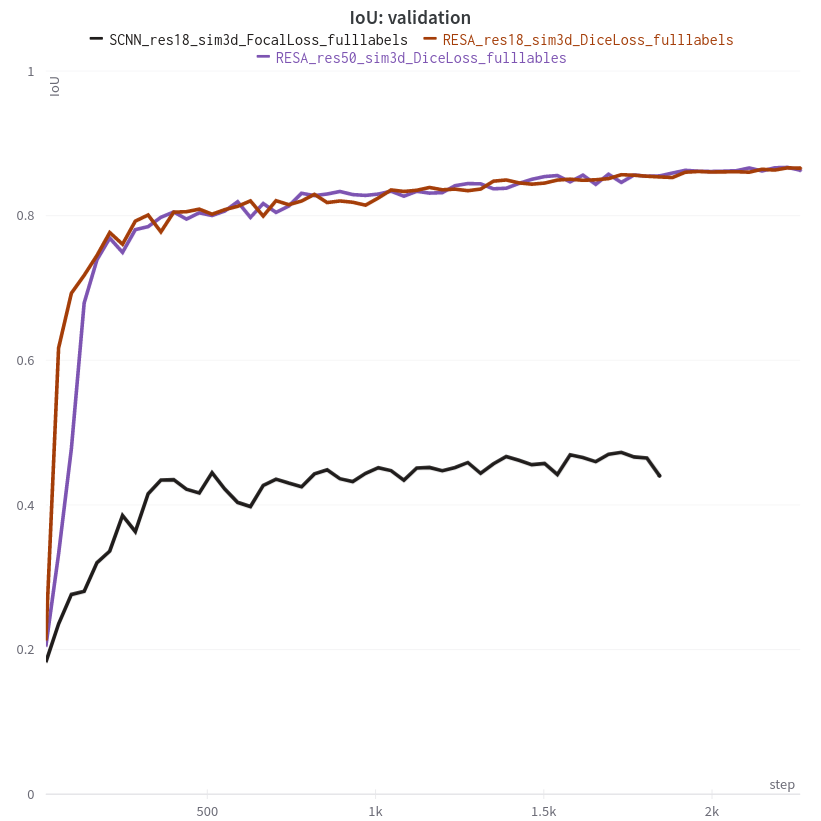
\includegraphics[scale=0.2]{images/change1.png}
\end{figure}

\end{frame}
%%%%%%%%%%5


\begin{frame}{Results: Gen-LaneNet Trained with Best Binary Lane Segmentation Model }
\begin{itemize}
    \item To prove the flexibility and efficacy of the dual stage approach proposed by Gen-LaneNet.
    \item The best binary segmentation model is used in the first step of the pipeline. 
    % \item First stage of the pipeline is frozen.
    \item The whole pipeline is trained on Apollo Synthetic dataset (Sim3D).
    \item The dataset is divided into three splits: balanced, rarely observed and visual variation scenes.
\end{itemize}
\end{frame}

%%%%%%%%%%%%%%

\begin{frame}{Comparison with SOTA: Balanced Scenes}
\begin{table}[h]
    \small
    \addtolength{\tabcolsep}{-1pt}
    \begin{center}
    \caption{Comparison between state of the art 3D lane detection approaches and the GenLaneNet trained with complex binary lane segmentation architecture on balanced scenes from sim3D , near range (0-40m) and far range (40-100m)}
    \begin{tabular}{|p{0.29\linewidth}|p{0.09\linewidth}|p{0.09\linewidth}|p{0.09\linewidth}|p{0.09\linewidth}|p{0.09\linewidth}|p{0.09\linewidth}|}
    \hline
        \textbf{Method} & \textbf{AP} & \textbf{F-Score} & \textbf{x error near(m)} & \textbf{x error far(m)} & \textbf{z error near(m)} & \textbf{z error far(m)} \\ \hline
        Gen-LaneNet & 90.1 & 88.1 & 0.061 & 0.496 & 0.012 & 0.214 \\ \hline
        3D LaneNet & 89.3 & 86.4 & 0.068 & 0.477 & 0.015 & \textbf{0.202} \\ \hline
        CLGo & \textbf{94.2} &\textbf{ 91.9} & 0.061 & \textbf{0.361} & 0.029 & 0.250 \\ \hline
        3D-LaneNet(1/att)  &  93.2 & 91.0 & 0.082 & 0.439 & \textbf{0.011} & 0.242 \\ \hline
        Gen-LaneNet(1/att)& 92.4 & 90.3 & 0.080 & 0.473 & \textbf{0.011} & 0.247 \\ \hline
        Gen-LaneNet(RESA+Res18) & 91.8 & 89.7 & \textbf{0.06} & 0.466 & 0.0114 & 0.24 \\ \hline
        Gen-LaneNet(RESA+Res50) & 92.2 & 90.2 &\textbf{ 0.06} & 0.461 & 0.0122 & 0.24 \\ \hline
    \end{tabular}
    \end{center}
    \end{table}

\end{frame}

%%%%%%
%qualitative results

\begin{frame}{Qualitative Results: Balanced Scenes}
 \begin{figure}[h]
      \caption{Qualitative results of the trained GenLaneNet trained with complex binary lane segmentation architecture on balanced scenes from sim3D dataset \footcite{guo2020gen} for uphill and downhill scenario. The ground-truth lines are color coded in red and the predicted lanes in blue. }
        \centering 
       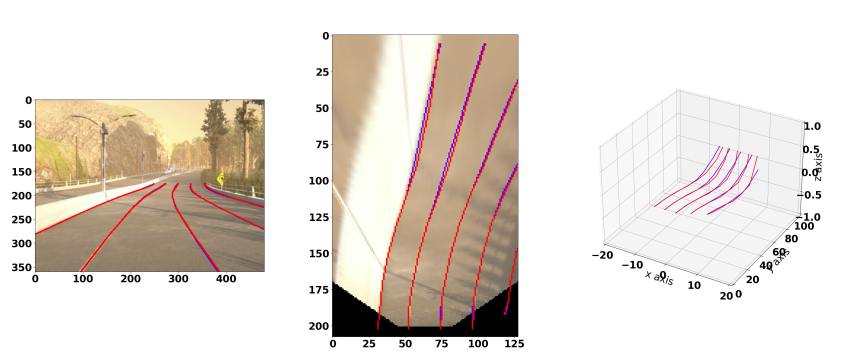
\includegraphics[scale=0.2]{images/uphill_standard.png}
       % \caption{(a)}
       \hfill
       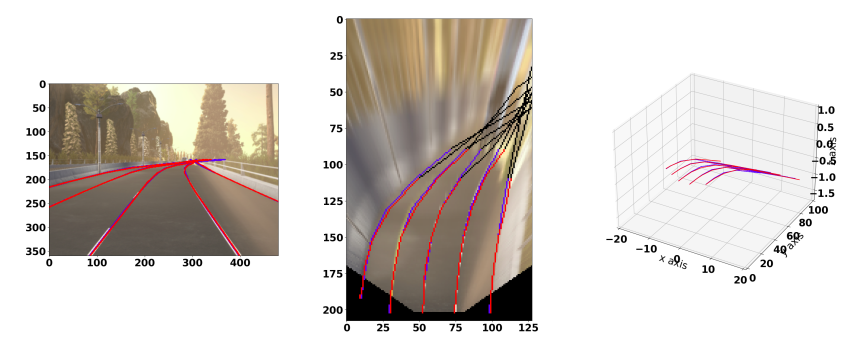
\includegraphics[scale=0.2]{images/downhill_standard.png}
        % \caption((b))
        \end{figure}
    
\end{frame}
%%%%%%%
%% table 
\begin{frame}{Comparison with SOTA: Rarely Observed Scenes}
     \begin{table}[h]
     \small
    \centering
    \caption{Comparison between state of the art 3D lane detection approaches and the GenLaneNet trained with complex binary lane segmentation architecture on rarely observed scenes from sim3D, near range (0-40m) and far range (40-100m) }
    \begin{tabular}{|p{0.29\linewidth}|p{0.09\linewidth}|p{0.09\linewidth}|p{0.09\linewidth}|p{0.09\linewidth}|p{0.09\linewidth}|p{0.09\linewidth}|}
    \hline
        \textbf{Method} & \textbf{AP} & \textbf{F-Score} & \textbf{x error near(m)} & \textbf{x error far(m)} & \textbf{z error near(m)} & \textbf{z error far(m)} \\ \hline
        Gen-LaneNet & 79.0 & 78.0 & 0.139 & 0.903 & 0.030 & 0.539 \\ \hline
        3D LaneNet & 74.6 & 72.0 & 0.166 & 0.855 & 0.039 &\textbf{ 0.521} \\ \hline
        CLGo &\textbf{ 88.3} &\textbf{ 86.1} & 0.147 & \textbf{0.735} & 0.071 & 0.609 \\ \hline
        3D-LaneNet(1/att)& 85.8 & 84.1 & 0.289 & 0.925 &\textbf{ 0.025} & 0.625 \\ \hline
        Gen-LaneNet(1/att)& 83.2 & 81.7 & 0.283 & 0.915 & 0.028 & 0.653 \\ \hline
        Gen-LaneNet(RESA+Res18) &  84.9 & 83.2 &\textbf{ 0.135} & 0.886 & 0.0308 & 0.607 \\ \hline
        Gen-LaneNet(RESA+Res50) & 83.7 & 82.3 & 0.14 & 0.919 & 0.0283 & 0.604 \\ \hline
    \end{tabular}
\end{table}
\end{frame}
%%%%
%%%% qualitative results 
\begin{frame}{Qualitative Results: Rarely Observed Scenes}

 \begin{figure}[h]
      \caption{Qualitative results of the GenLaneNet trained with complex binary lane segmentation architecture on rarely observed scenes from sim3D dataset\footcite{guo2020gen} for uphill and downhill scenario. The ground-truth lines are color-coded in red and the predicted lanes in blue.}
        \centering
        
        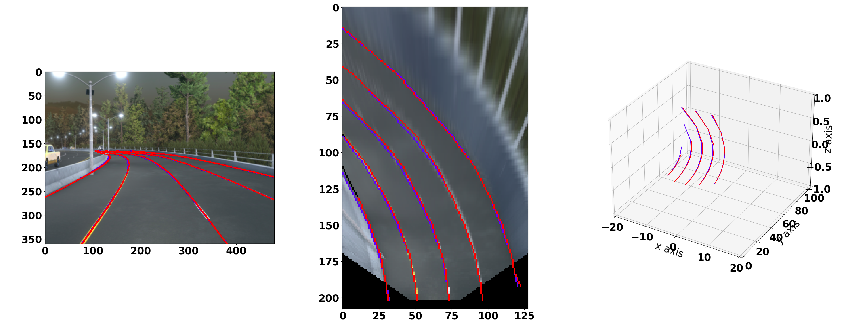
\includegraphics[scale=0.2]{images/uphill_rare.png} 
        \hfill
        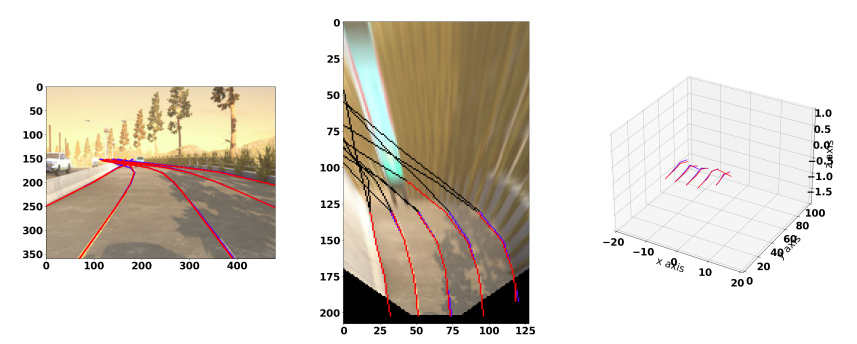
\includegraphics[scale=0.2]{images/downhill_rare.png}
       
        \end{figure}
    
\end{frame}
%% table 
\begin{frame}{Comparison with SOTA: Visual Variation Scenes}
      \begin{table}[h]
      \small
    \centering
    \caption{Comparison between state of the art 3D lane detection approaches and the GenLaneNet  trained with complex binary lane segmentation architecture on scenes with visual variations from sim3D, near range (0-40m) and far range (40-100m)}
    \begin{tabular}{|p{0.29\linewidth}|p{0.09\linewidth}|p{0.09\linewidth}|p{0.09\linewidth}|p{0.09\linewidth}|p{0.09\linewidth}|p{0.09\linewidth}|}
    \hline
        \textbf{Method} & \textbf{AP} & \textbf{F-Score} & \textbf{x error near(m)} & \textbf{x error far(m)} & \textbf{z error near(m)} & \textbf{z error far(m)} \\ \hline
        Gen-LaneNet & 87.2 & 85.3 & 0.074 & 0.538 & 0.015 & 0.232 \\ \hline
        3D LaneNet & 74.9 & 72.5 & 0.115 & 0.601 & 0.032 & \textbf{0.230} \\ \hline
        CLGo & 89.2 & 87.3 & 0.084 & \textbf{0.464} & 0.045 & 0.312 \\ \hline
        3D-LaneNet(1/att) & 87.4 & 85.4 & 0.118 & 0.559 & 0.018 & 0.290 \\ \hline
        Gen-LaneNet(1/att) & 88.5 & 86.8 & 0.104 & 0.544 & 0.016 & 0.294 \\ \hline
        Gen-LaneNet(RESA+Res18) & \textbf{ 91.1} &\textbf{ 89.2} & 0.734 & 0.496 & \textbf{0.0134} & 0.259 \\ \hline
        Gen-LaneNet(RESA+Res50) & 90.7 & 88.8 & \textbf{0.0653} & 0.477 & 0.014 & 0.258 \\ \hline
    \end{tabular}
\end{table}
\end{frame}
%%% Qualitative results
\begin{frame}{Qualitative Results: Visual Variation Scenes}
    \begin{figure}[h]
      \caption{Qualitative results of the  GenLaneNet trained with complex binary lane segmentation architecture on visually varied scenes from sim3D dataset\footcite{guo2020gen} for uphill and downhill scenario. The ground-truth lines are color-coded in red and the predicted lanes in blue.}
        \centering
        % \begin{subfigure}{1\textwidth}
        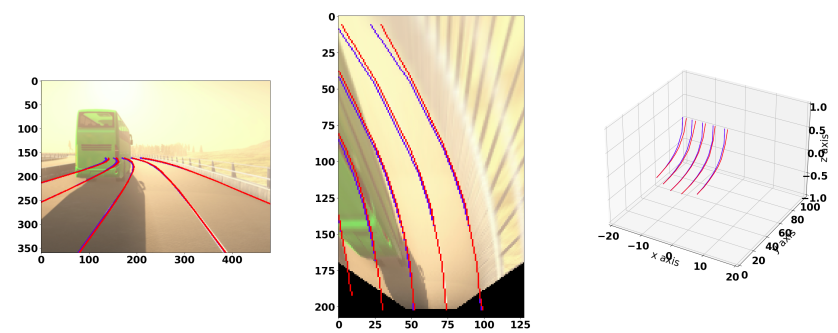
\includegraphics[width= 0.45\textwidth]{images/uphill_illus.png} 
        \hfill
        % \caption{\cite{guo2020gen}}
        % \label{fig:subim1}
        % \end{subfigure}
        % \begin{subfigure}{1\textwidth}
        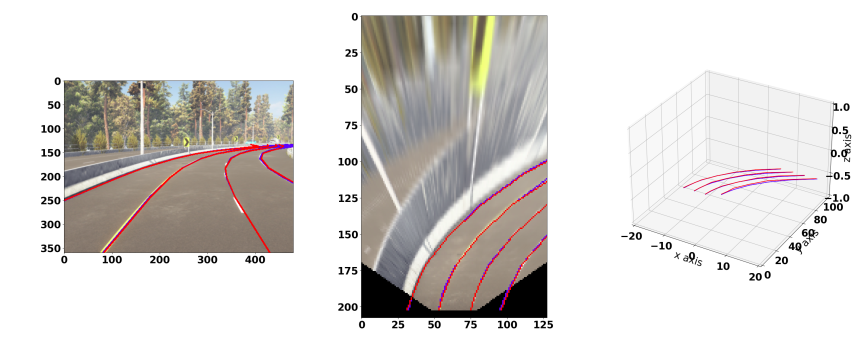
\includegraphics[width= 0.45\textwidth]{images/downhill_illus.png}
        % \caption{\cite{guo2020gen}}
        % \label{fig:subim2}
        % \end{subfigure}
        \end{figure}
\end{frame}

%%%%%%%%%%%%% STAGE 2

\begin{frame}{Stage 2: Anchor Less Semi-local 3D Lane Detection}
     \begin{figure}[H]
     \centering
     
%\begin{subfigure}{\textwidth}
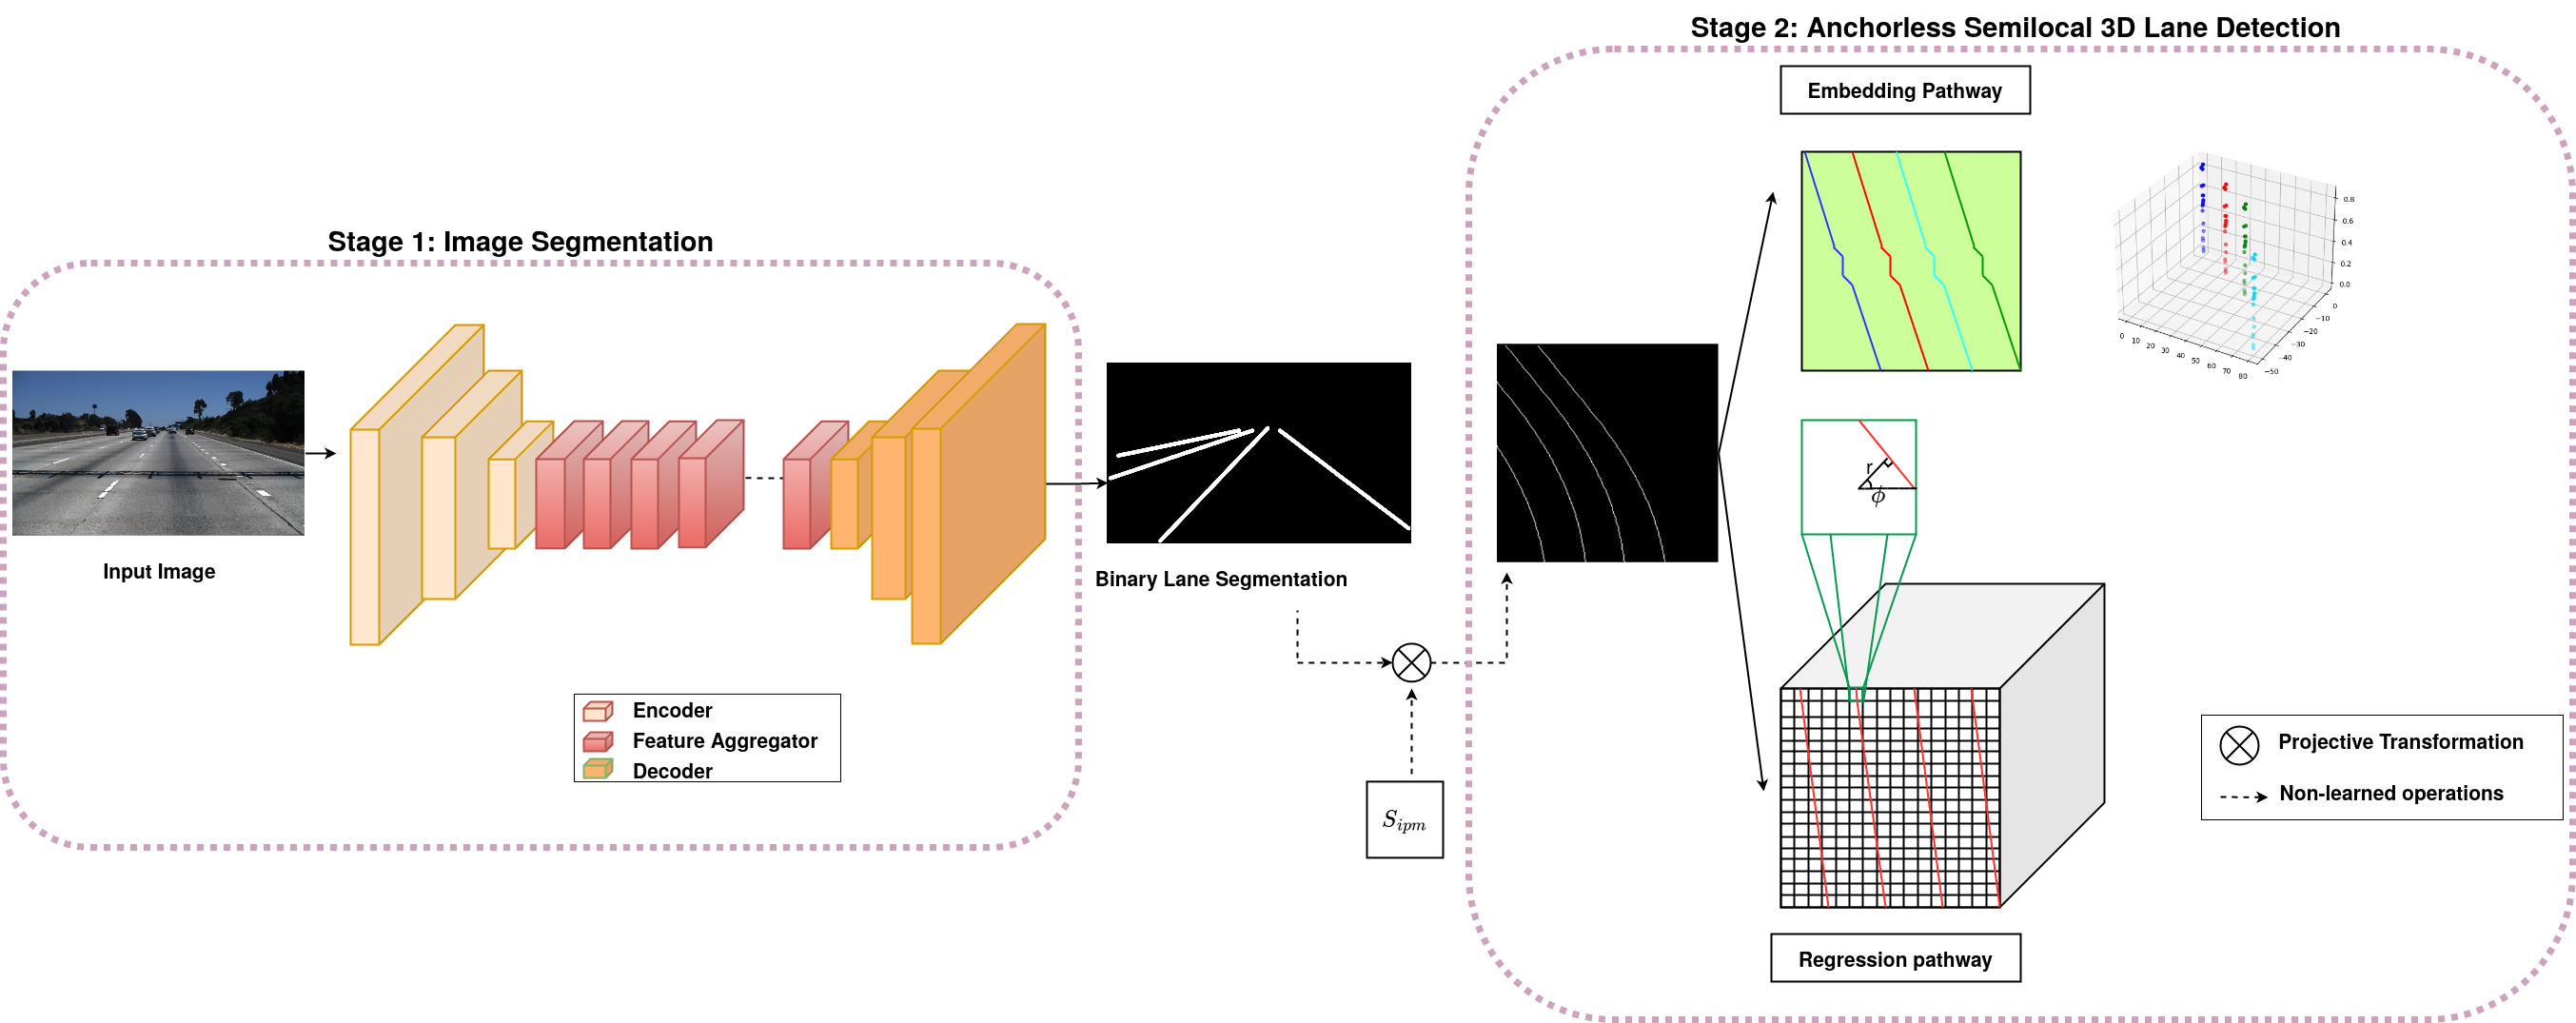
\includegraphics[width=0.8\linewidth, height=4.5cm]{images/3DlaneAUXNet.png} 
\label{fig:subim1}
%\end{subfigure}

\caption{Dual stage semi-local anchor-less 3D lane detection pipeline }
\label{fig:image2}
\end{figure}
\end{frame}

\begin{frame}{Stage 2: Anchor Less Semi-local 3D Lane Detection}
\begin{itemize}
    \item Binary segmentation mask is transformed into birds-eye-view using projective transformation.
    \item Second stage consists of two pathways: regression and embedding pathway.
    \item Regression pathway is responsible for extracting geometric information for 3D lane curves.
    \item Embedding pathway is responsible for assigning clusters to the lane line points.
    \item All the regressed geometric parameters are converted into 3D real world points and labels are assigned to them for visualization.
\end{itemize}
\end{frame}

\begin{frame}{Regression Pathway}    
    \begin{itemize}
        \item The BEV segmentation mask is normalized.
        \item Resulting BEV segmentation mask is decimated into grids $G_{WxH}$, which are non overlappig patches called tiles and passed through series of convolutional layers.
        \item Every tile contributes one point to the 3D lane curve.
        \item For each tile we try to approximate a straight line segment assuming it intersects a tile.
        \item For each tile the regression pathway regresses, $\widetilde{r_{ij}}$ the lateral offset distance relative to tile center, line angle $\widetilde{\phi_{ij}}$, $\triangle{\widetilde{z_{ij}}}$ and a binary classification score $\widetilde{c_{ij}}$ 
    \end{itemize}
    
\end{frame}

\begin{frame}{Ground-truth Creation: Regression Pathway}
    \begin{itemize}
        \item  Ground-truth for angle and distance offsets are computed by projecting ground-truth 3D lane points on the road plane in BEV space.
        \item Projected BEV image is decimated into tiles.
        \item Line approximation algorithms like Hough Transform is used to compute $r_{ij}$ and $\phi_{ij}$.
        \item This is done for all decimated tiles
        \item To represent the line angle distance offsets with respect to the global origin of the image, Hesse normal form is used.
    \end{itemize}

     
\end{frame}

\begin{frame}{Ground-truth Creation: Regression Pathway}
    \begin{figure}[h]
      \caption{Height offset is calculated by considering two scenarios.}
        \centering
        % \begin{subfigure}{1\textwidth}
        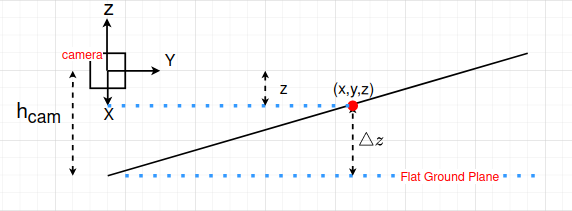
\includegraphics[scale=0.2]{images/delta_z_uphill.png} 
        % \hfill
        % \caption{\cite{guo2020gen}}
        % \label{fig:subim1}
        % \end{subfigure}
        % \begin{subfigure}{1\textwidth}
        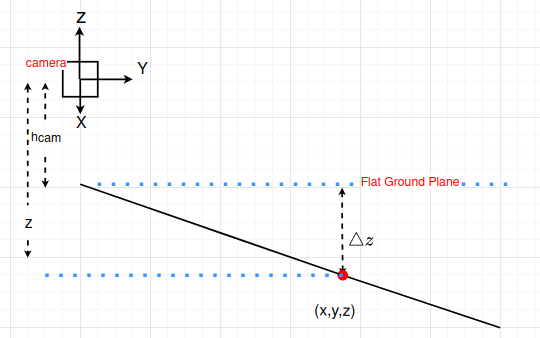
\includegraphics[scale=0.2]{images/delat_z_downhill.png}
        % \caption{\cite{guo2020gen}}
        % \label{fig:subim2}
        % \end{subfigure}
        \end{figure}
\end{frame}

\begin{frame}{Loss Functions: Regression Pathway}
    \begin{itemize}
        \item L1 loss is used to train position and angle offset
    \end{itemize}
    
    \begin{equation}
                L^{Offsets}_{i,j} = \parallel \widetilde{r_{i,j}} - r_{i,j} \parallel_{1} + \parallel \triangle{\widetilde{z_{i,j}}} - \triangle{z_{i,j}} \parallel_{1} 
     \end{equation}

    \begin{itemize}
        \item Prediction of $\widetilde{\phi}_{ij}$ is carried out by representing it in the form of histogram of $N_{\alpha}$ bins, where $\alpha = \left\{\frac{2\pi}{N_{\alpha} } \cdot i \right\}^{N_{\alpha}}_{i =1} $.
        \item Ground-truth probability of each bin is calculated via $ p^{\alpha} = [1 - \vert \frac{2\pi}{N_{\alpha}} \cdot i  - \phi  \vert \ \frac{2\pi}{N_{\alpha}} ]_{+}$
        \item $\triangle_{\alpha}$ is learned to counter the bin classification offsets.
        \item Angle loss is the combination of classification and regression losses.
    \end{itemize}

    \begin{equation}
                 L_{ij}^{Offsets} = \sum_{\alpha=1}^{N_{\alpha}}[p^{\alpha}_{ij} \cdot log \tilde{p^{\alpha}_{ij}} + (1 - p^{\alpha}_{ij}) \cdot log(1 - \tilde{p^{\alpha}_{ij}}) + \delta^{\alpha}_{ij} \parallel   \tilde{\triangle^{\alpha}_{ij}} - \triangle^{\alpha}_{ij} \parallel_{1} ] 
             \end{equation}
    
\end{frame}

\begin{frame}{Loss Functions: Regression Pathway}
    \begin{itemize}
        \item Lane tile probability is traned via binary cross entropy loss.
    \end{itemize}
    \begin{equation}
                 L_{ij}^{score} = c_{ij} \cdot log \widetilde{c_{ij}} + (1 - c_{ij}) \cdot log
                    (1-  \widetilde{c_{ij}})
             \end{equation}

    \begin{itemize}
        \item Overall tile loss is sum of all above mentioned losses for all tiles in the grid.
    \end{itemize}

     \begin{equation}
                L^{tiles} = \sum_{i,j \in WxH}(L^{score}_{ij} +c_{ij} \cdot L^{angle}_{ij} + c_{ij} \cdot L^{offsets}_{ij}  )
            \end{equation}
    
\end{frame}

\begin{frame}{Embedding Pathway}
\begin{itemize}
    \item The normalized BEV mask is passed through series of $1x1$ convolutional layers to learn global lane embeddings.
    \item For each tile an embedding vector $f_{ij}$ is learned which is governed by a discriminative push-pull loss.
    \item Mean shift clustering is performed on the learnt feature embeddinds to complete the lane segments to complete lane curve.
\end{itemize}
\end{frame}

\begin{frame}{Loss functions: Embedding Pathway}
\begin{itemize}
    \item Discriminative push-pull loss make sures that embedding vectors that belong to same lane reside close to each other in embedding space.
    \item Embedding vectors which belong to different lane stay apart in embedding space. 
\end{itemize}
 \begin{equation}
                L^{embedding} = L^{pull} + L^{push}
            \end{equation}
             
             \begin{equation}
                     L^{pull} = \frac{1}{C} \sum^{C}_{c=1}\frac{1}{N_{c}} \sum_{ij \in WXH}[ \delta_{ij}^{c} \parallel \mu_{c} - f_{ij}  \parallel - \triangle_{pull} ]_{+}^{2} 
             \end{equation}
             
             \begin{equation}
                 L^{push} =  \frac{1}{C(C -1)} \sum^{C}_{C_{A=1}, C_{B=1}, C_{A} \not =C_{B}}[ \triangle_{push} - \parallel \mu_{CA} - \mu_{CB}\parallel ]_{+}^{2}
             \end{equation}
    \tiny
    where, $C$ is the number of lanes, $N_{c}$ number of tiles that belong to lane c, $\delta_{ij}^{c}$ denotes if tile $i,j$ belongs to lane c, $\mu_{c} = \frac{1}{N_{c}} \sum_{ij \in WXH } \delta^{c}_{ij} \cdot f_{ij}$ are mean of embedding vectors that belongs to lane $c$. $\triangle_{pull}$ and $\triangle_{pull}$ is the maximum and minimum distance between the clusters.
\end{frame}


\begin{frame}{Final Output}
    \begin{itemize}
        \item Mean shift clustering is performed on the learnt feature embedding to assign clusters to each tile.
        \item Predicted offsets and angles are converted into 3D lane line points by converting them from polar to cartesian coordinates.
        \item Resulting points are transformed from BEV to Camera coordinate system by rotating by  $-\theta_{cam}$ and subtracting by $h_{cam}$
    \end{itemize}

    \begin{equation}
            \begin{bmatrix}\widetilde{x_{ij}}  \\\widetilde{y_{ij}} \\ \widetilde{z_{ij}}  \end{bmatrix} = \begin{bmatrix}1 & 0 & 0  \\ 0  & cos(\theta_{cam}) & sin(\theta_{cam}) \\ 0  & -sin(\theta_{cam}) & cos(\theta_{cam}) \end{bmatrix} \cdot \begin{bmatrix}\widetilde{r_{ij}} \cdot cos(\widetilde{\phi_{ij}})  \\\widetilde{r_{ij}} \cdot sin(\widetilde{\phi_{ij}})  \\ \widetilde{\triangle z_{ij}} - h_{cam} \end{bmatrix}
        \end{equation}
\end{frame}

\begin{frame}{Training Challenges Encountered: Proposed Pipeline (1/3)}
    \begin{itemize}
        \item While training for both pathways together, magnitude of loss from Regression pathway is relatively greater than the other one. 
        \item Embedding pathway was not able to learn properly.
        \item Overall loss: \textbf{Iteration 1}
        \begin{equation}
    Overall loss = L_{regression} + L_{embedding} 
\end{equation}
        \item Overall loss: \textbf{Iteration 2}
        \begin{equation}
    Overall loss = w_{regression} * L_{regression} + w_{embedding} * L_{embedding} 
        \end{equation}
        \item Both iterations did not work for combined training of both pathways.
        \item Later both branches are learned independently. 
        \item Network was able to learn meaningful information.
    \end{itemize}
        

\end{frame}

\begin{frame}{Training Challenges Encountered: Proposed Pipeline (2/3)}

\begin{figure}[h]
      
        \centering
        % \begin{subfigure}{\textwidth}
        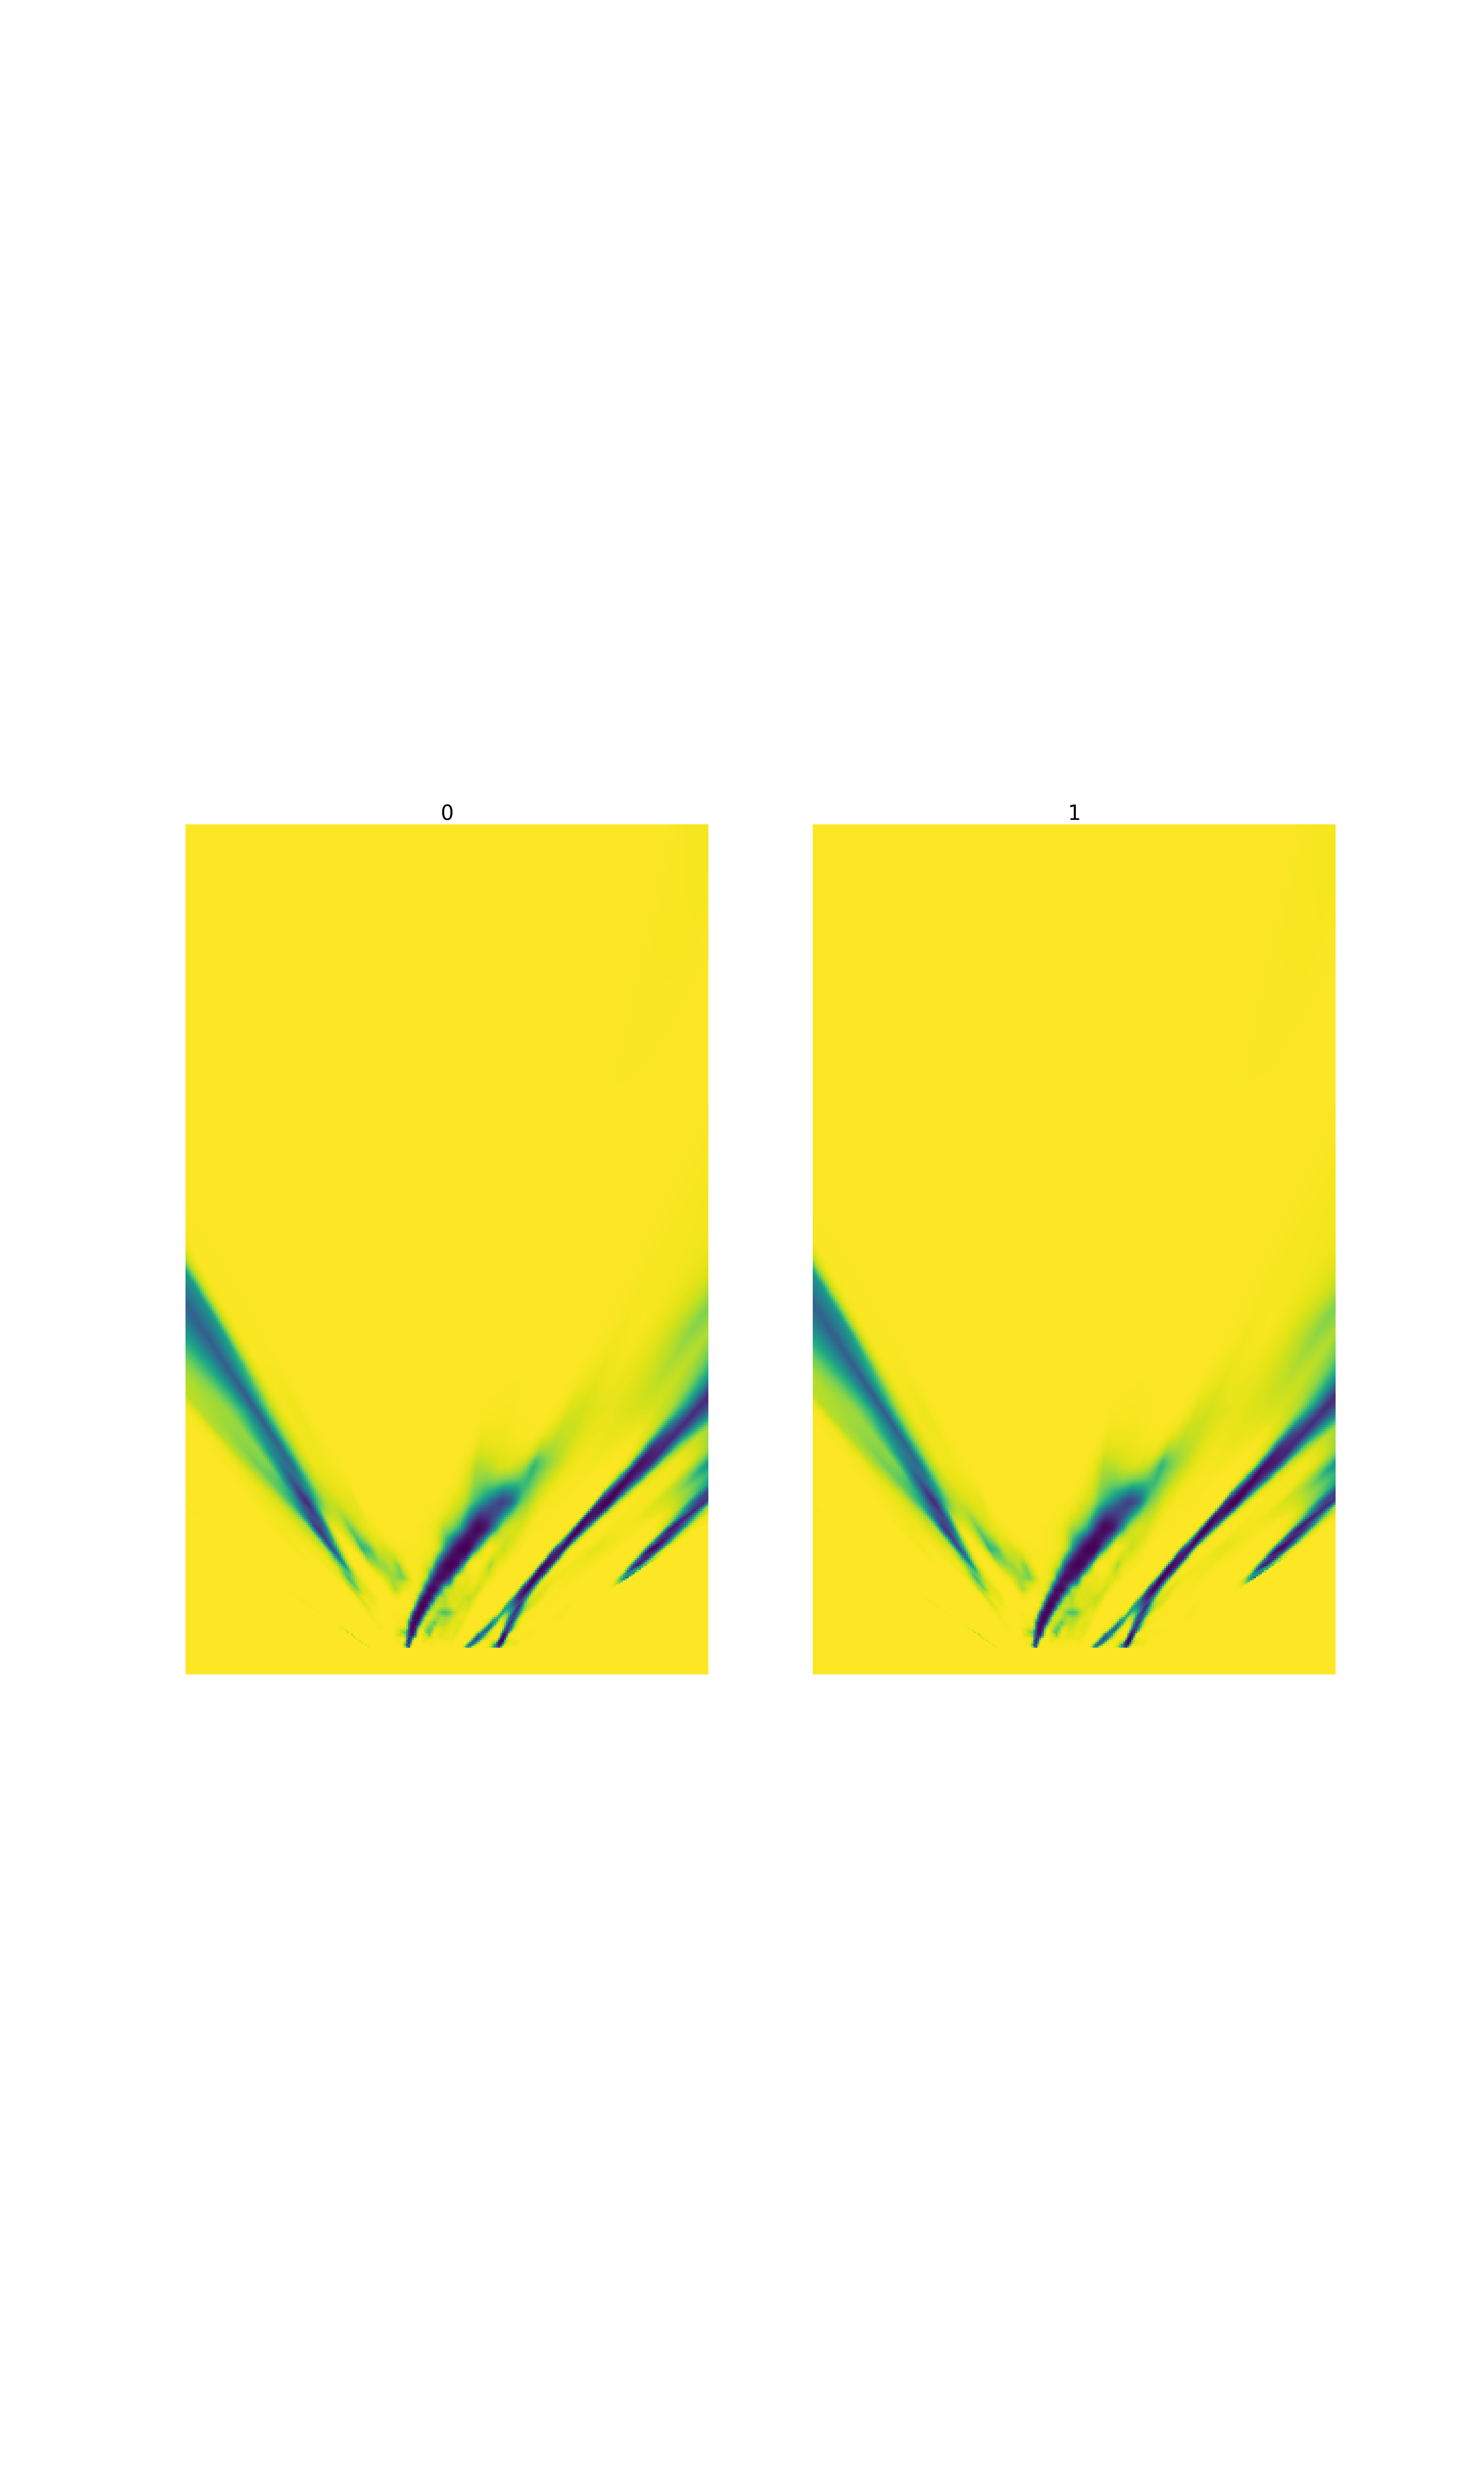
\includegraphics[width=0.4\linewidth, height=5cm]{images/activation_embededing_nofix.png} 
        % \label{fig:subim1}
        % \end{subfigure}
        % \begin{subfigure}{\textwidth}
        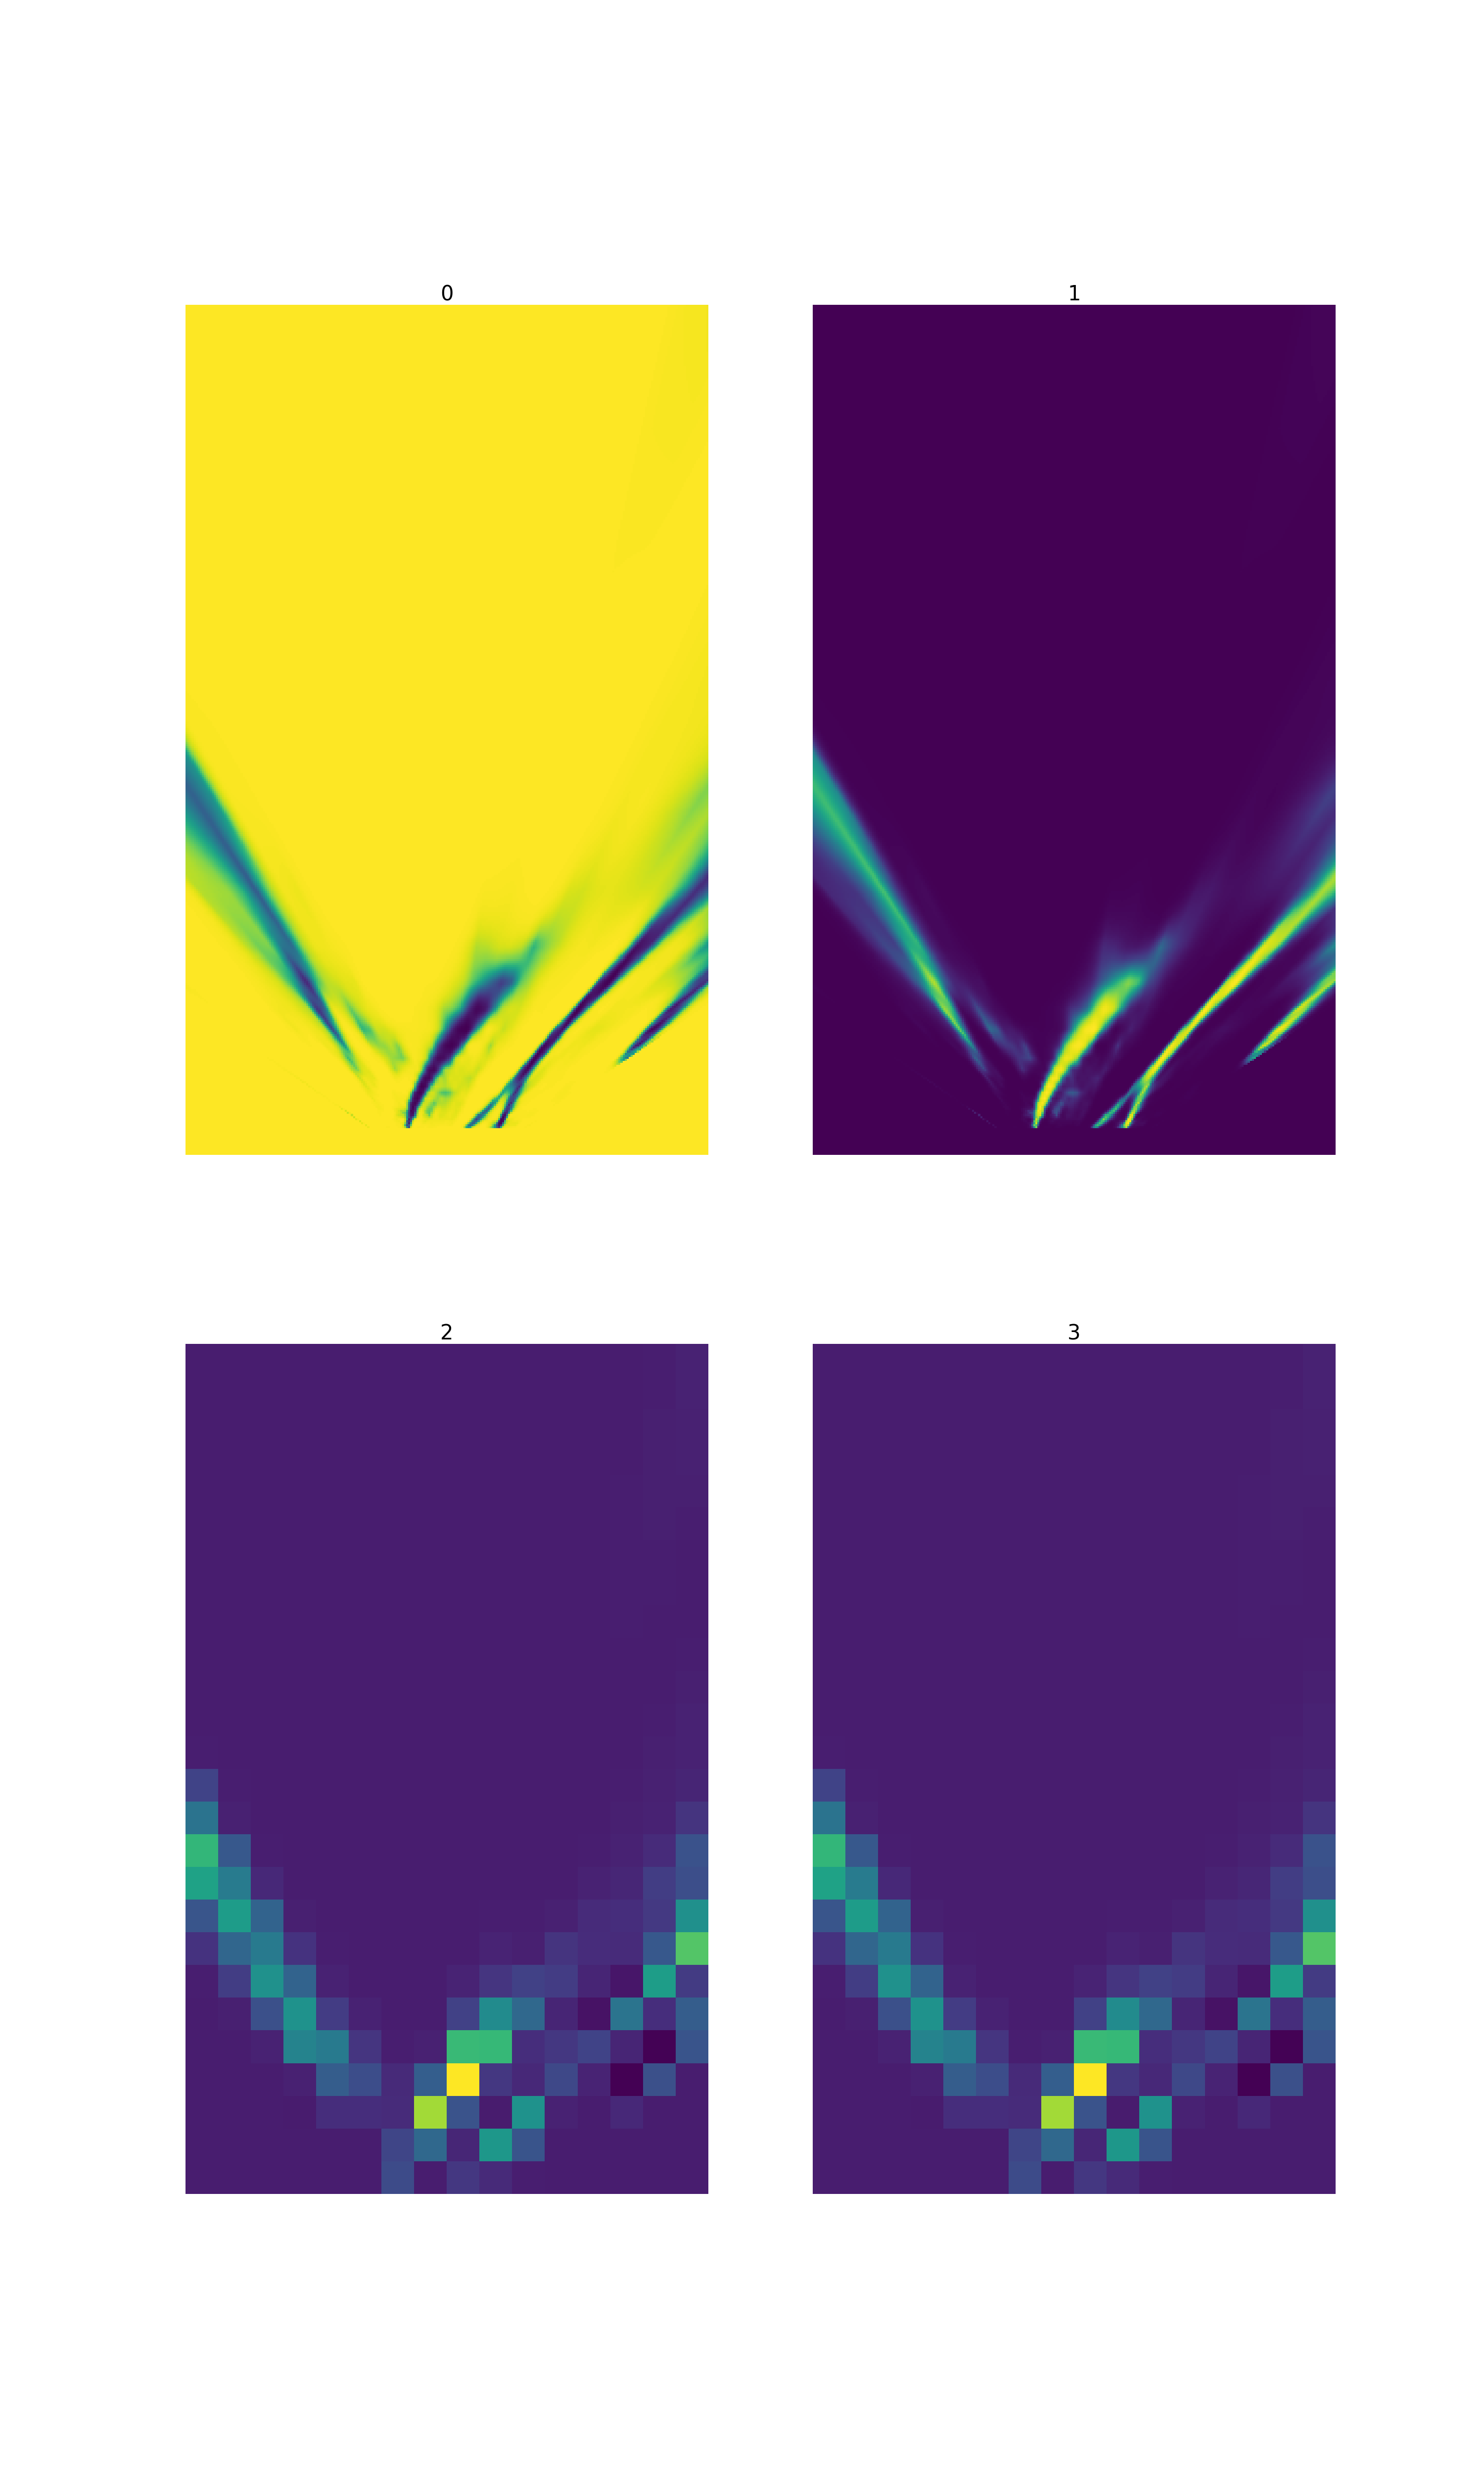
\includegraphics[width=0.4\linewidth,height=5cm]{images/embedding_regression_nofix.png}
        \caption{Activation maps of convolutional layers (a) embedding pathway (b) regression pathway, while training them simultaneously}
        % \caption{}
        % \label{fig:subim2}
        % \end{subfigure}
        \end{figure}
\end{frame}

\begin{frame}{Training Challenges Encountered: Proposed Pipeline (3/3)}

\begin{figure}[h]
      
        \centering
        % \begin{subfigure}{\textwidth}
        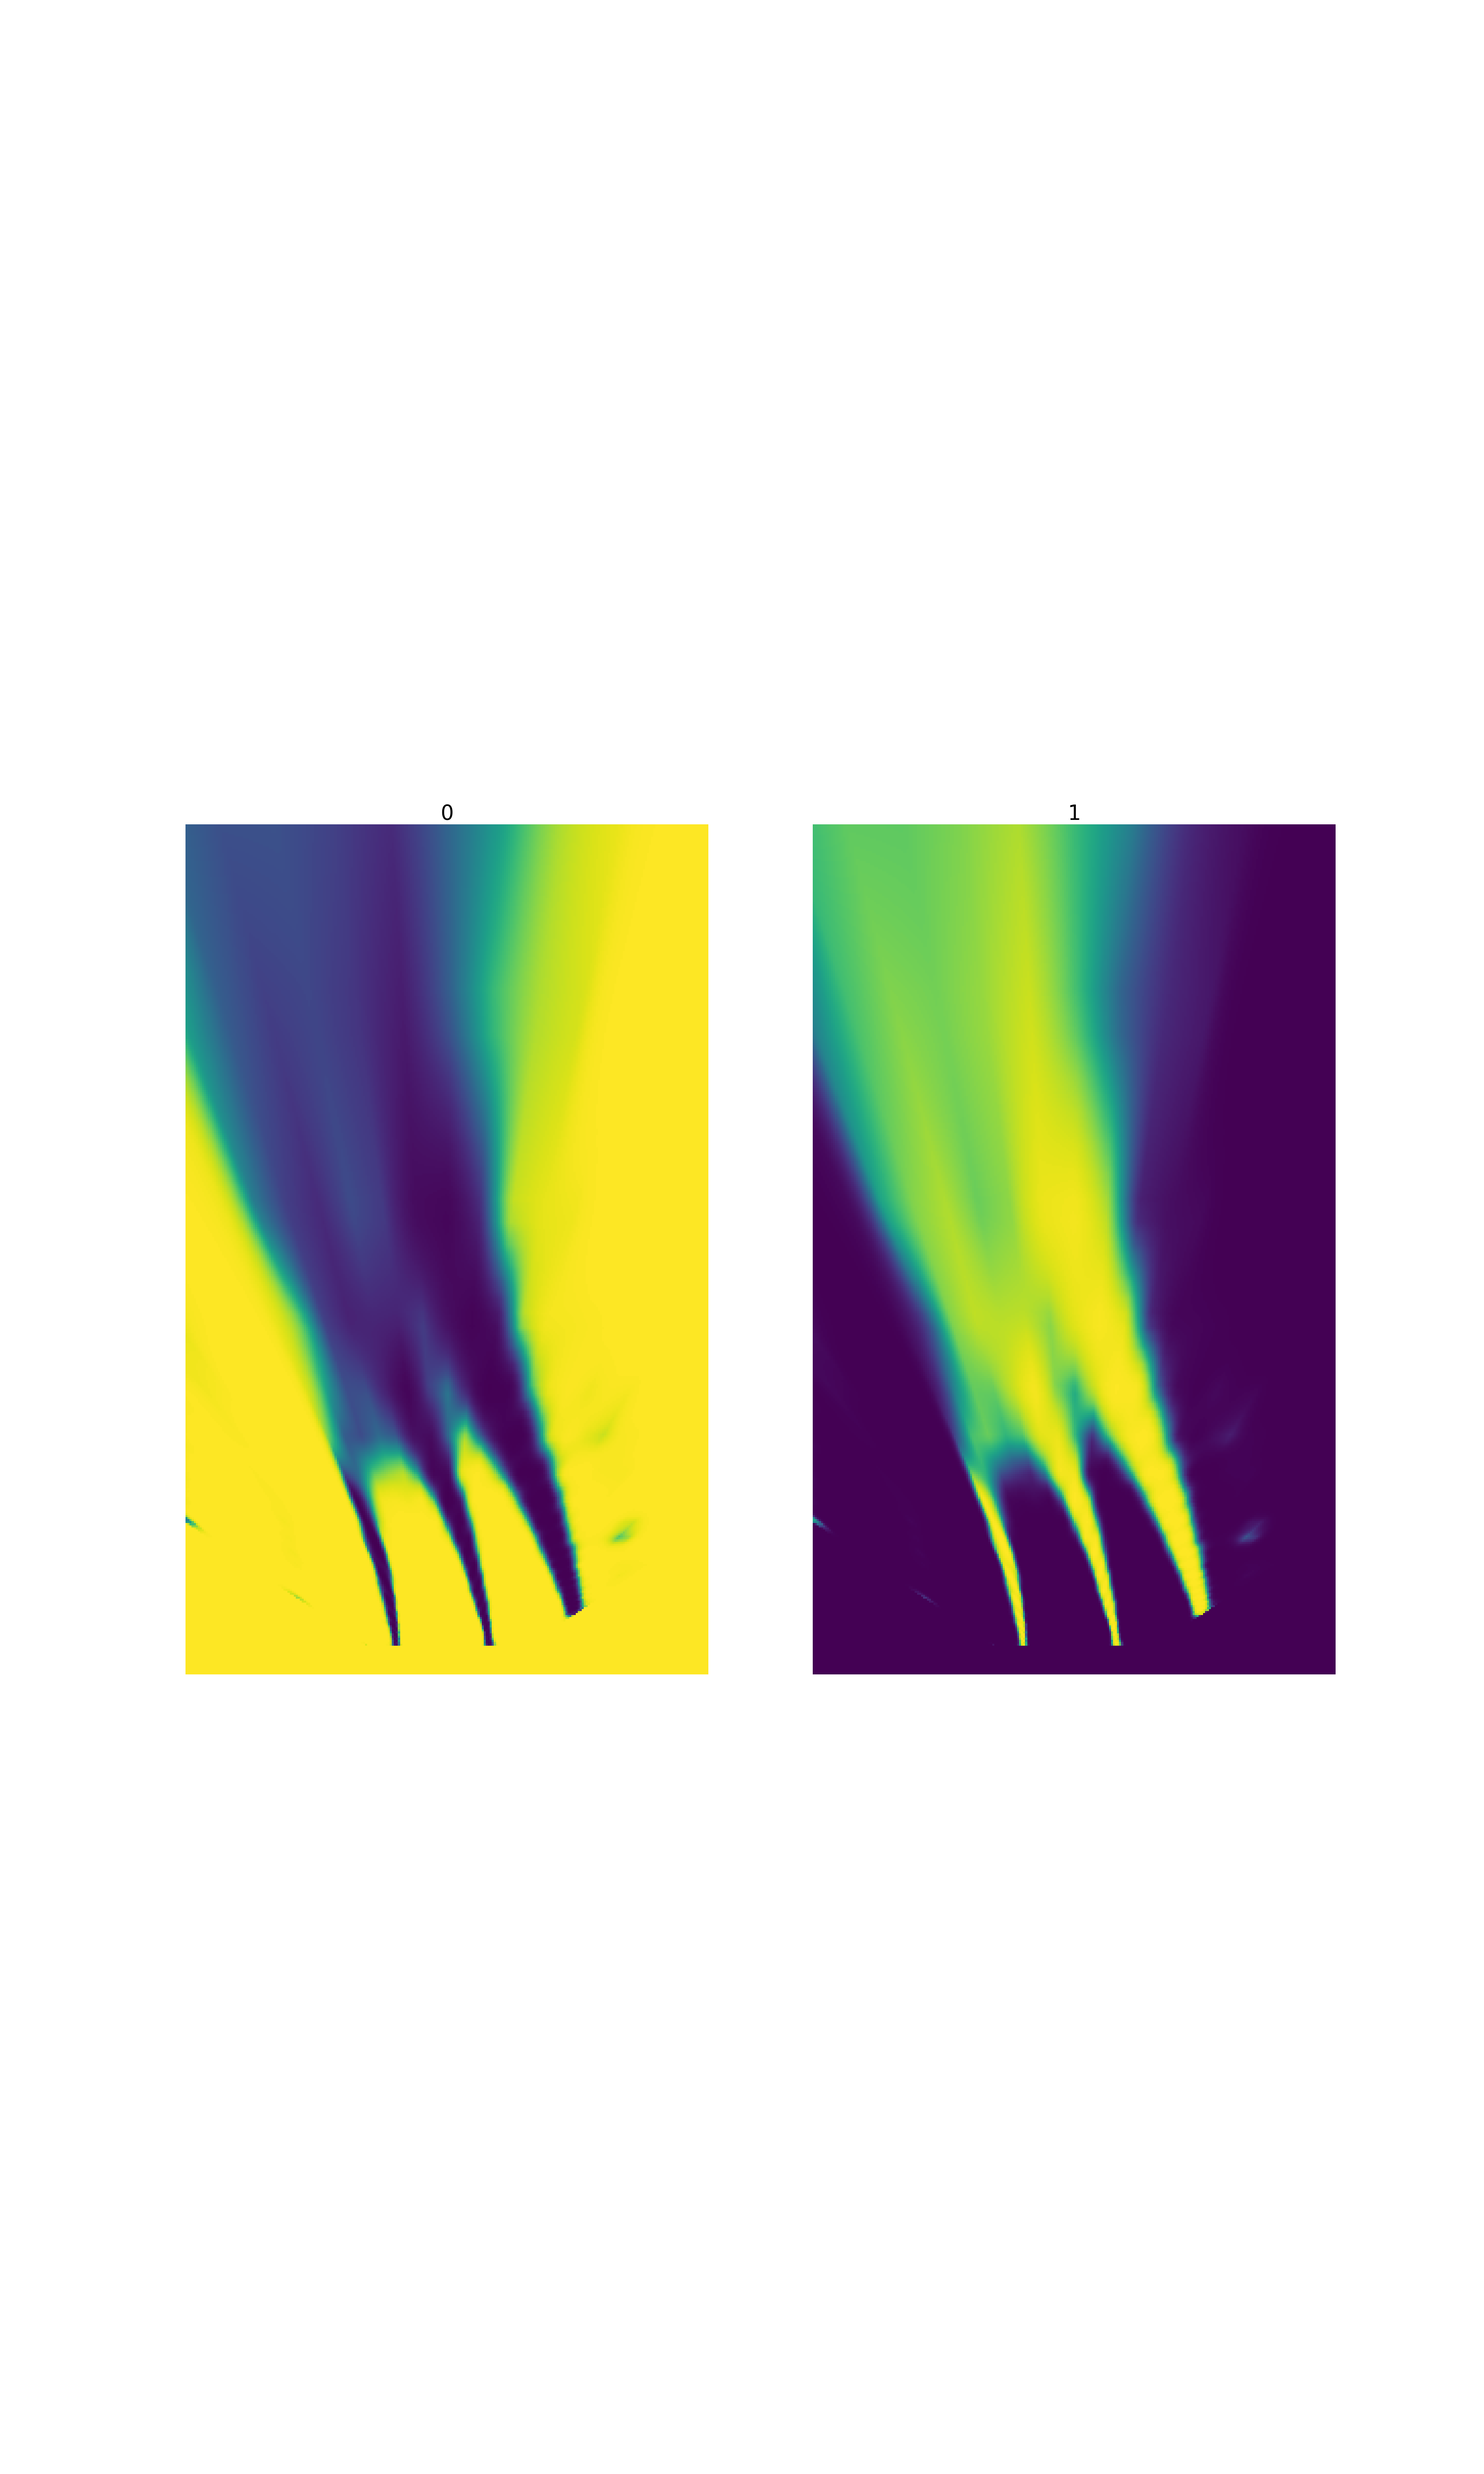
\includegraphics[width=0.4\linewidth, height=5cm]{images/activation_embedding.png} 
        % \label{fig:subim1}
        % \end{subfigure}
        % \begin{subfigure}{\textwidth}
        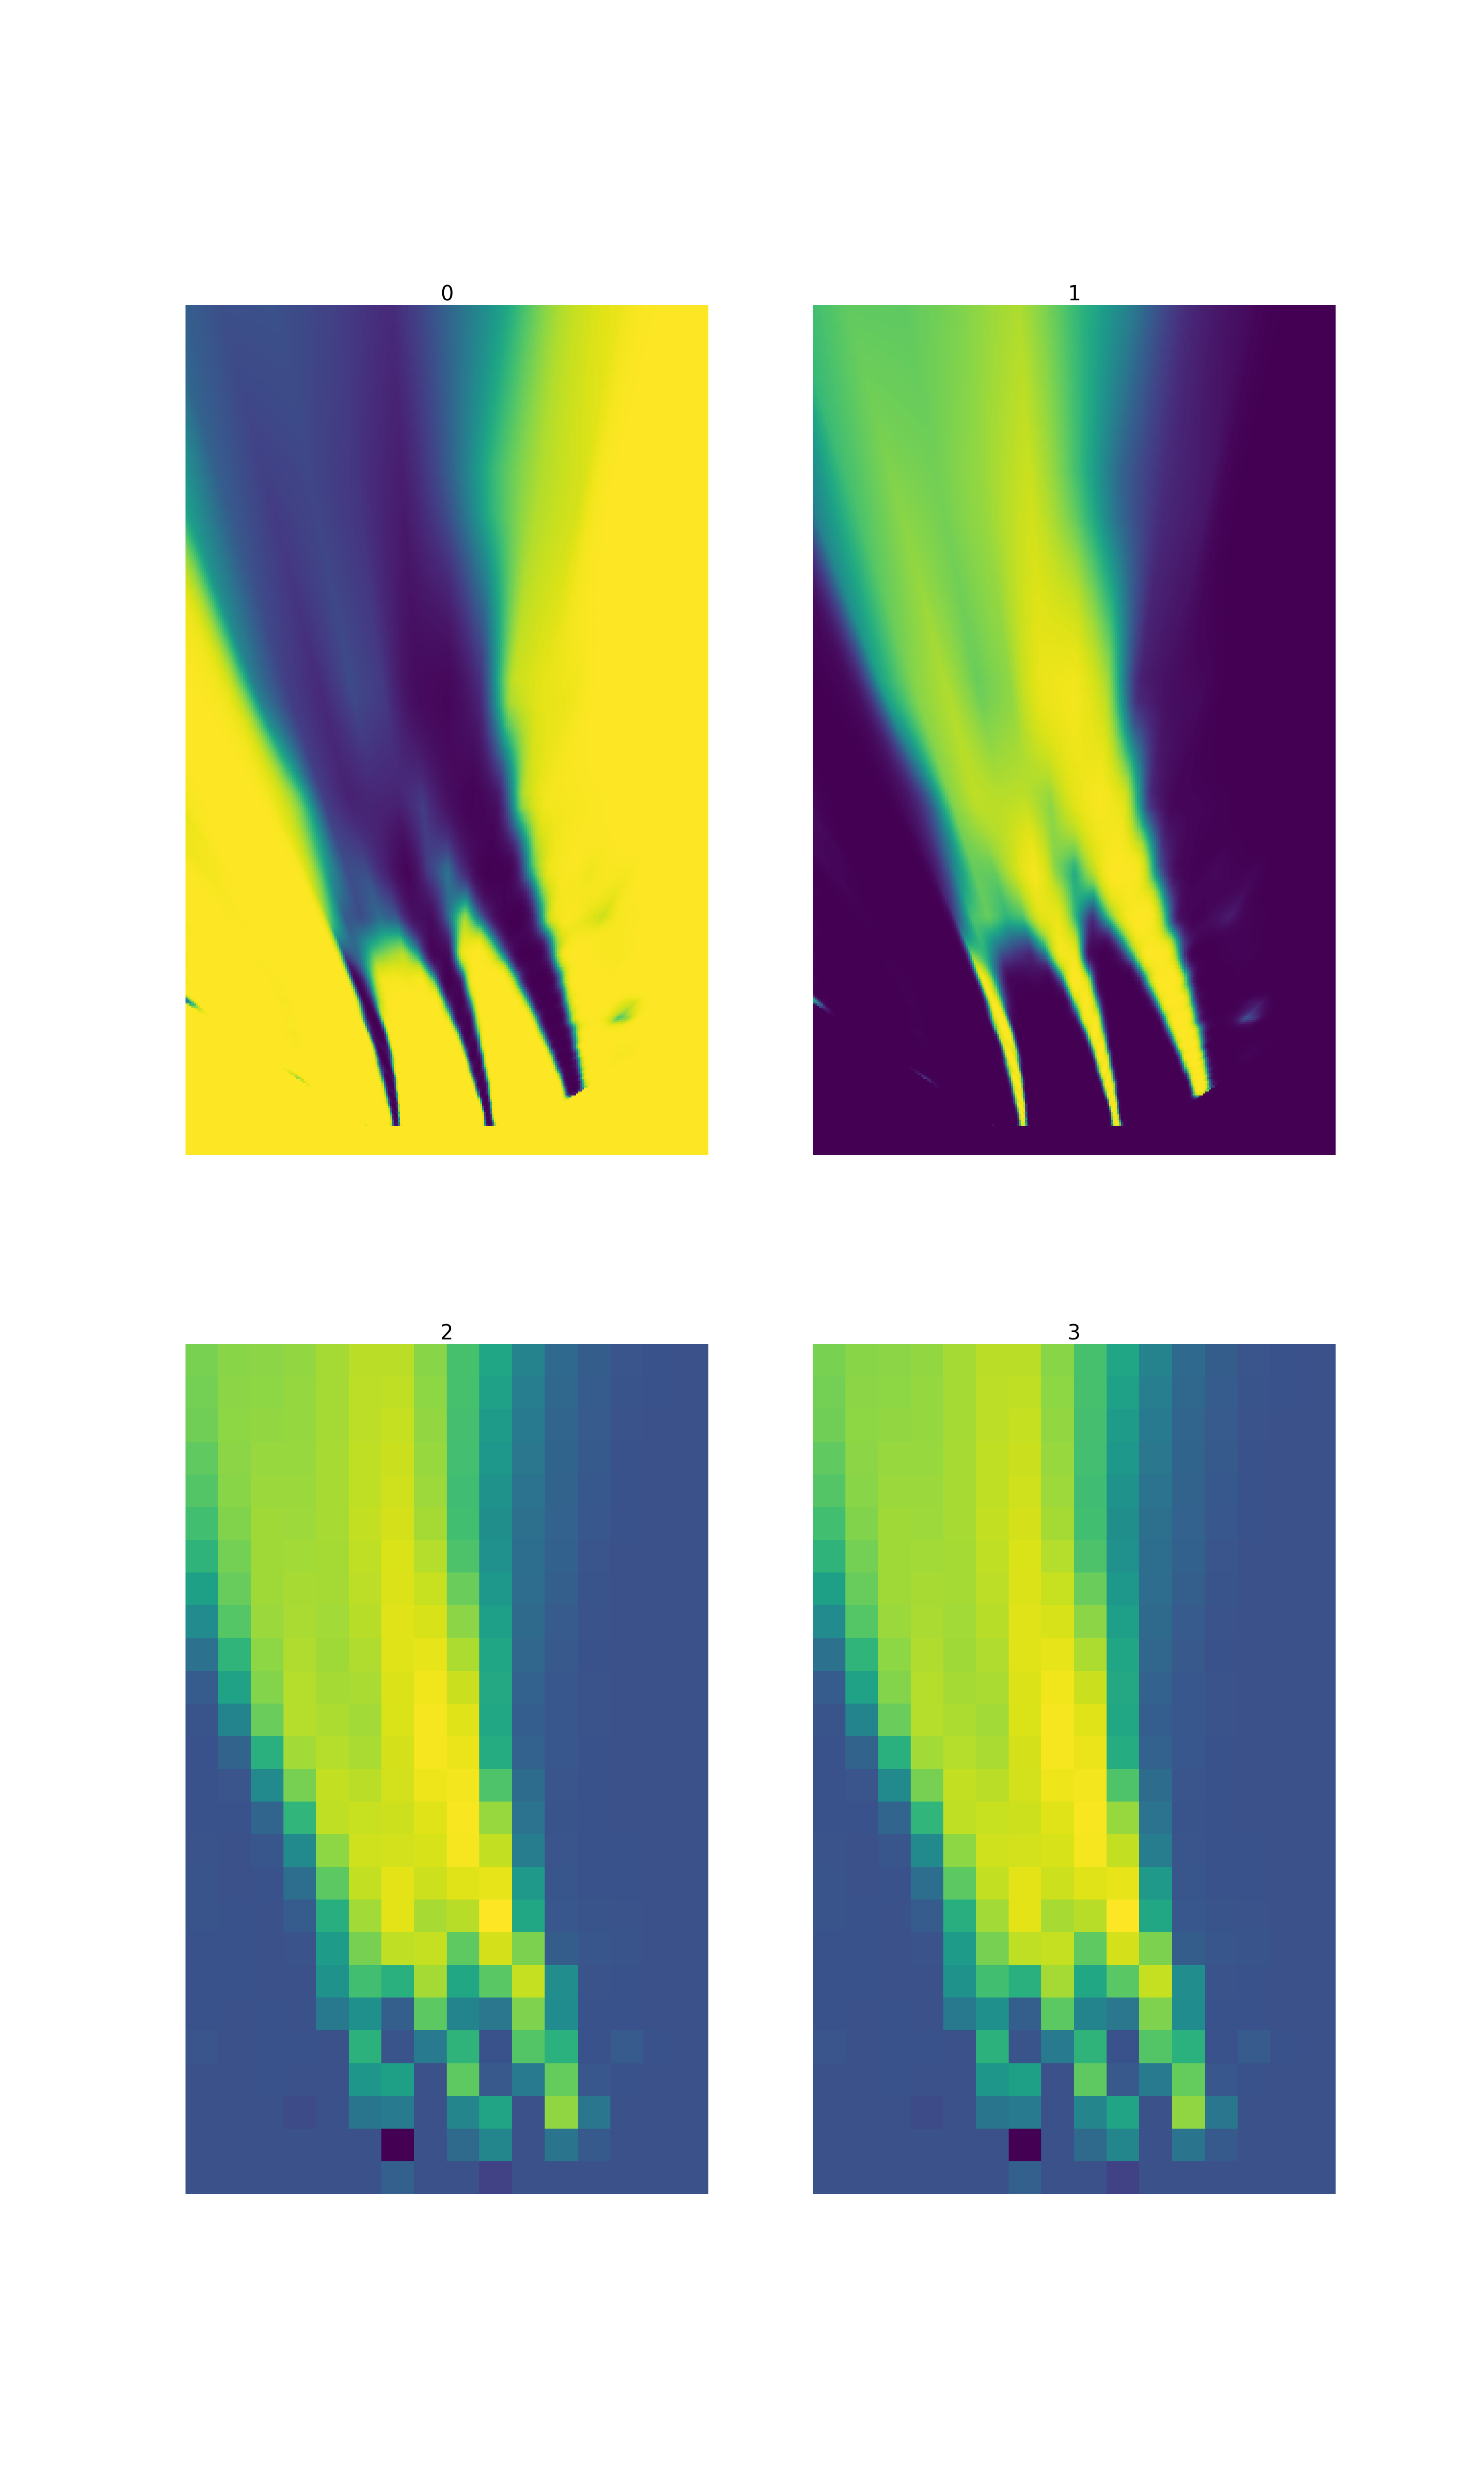
\includegraphics[width=0.4\linewidth,height=5cm]{images/activation_regression.png}
        \caption{Activation maps of convolutional layers (a) embedding pathway (b) regression pathway, while training them independently}
        % \caption{}
        % \label{fig:subim2}
        % \end{subfigure}
        \end{figure}
\end{frame}

\begin{frame}{Challenges: Proposed Pipeline}
    \begin{itemize}
        \item Ground-truth for regressed geometric parameter were not computed properly.
        \item 3D lane curves are traced back from the groundturth geometric parameters for all tiles in a scene using equation 13 were not meaningful.
        % \item Viusalization does not make any sense.
        \item Correctness of the geometric parameters obtained by Hough Transform is validated for a single tile and visualized.
        \item Later it is done for all the tiles and the lane curves are traced back.
        \item To validate the speculation that the geometric parameters are calculated in the vicinity of tile itself, they are represented in terms of a global origin of the image using Hesse normal form.
        \item Visualizations validated that the geometric parameters are computed correctly.
    \end{itemize}
\end{frame}
%------------------
\begin{frame}{Validating Hough Transform (1/2)}
    \begin{figure}[h]
      
        \centering
        % \begin{subfigure}{\textwidth}
        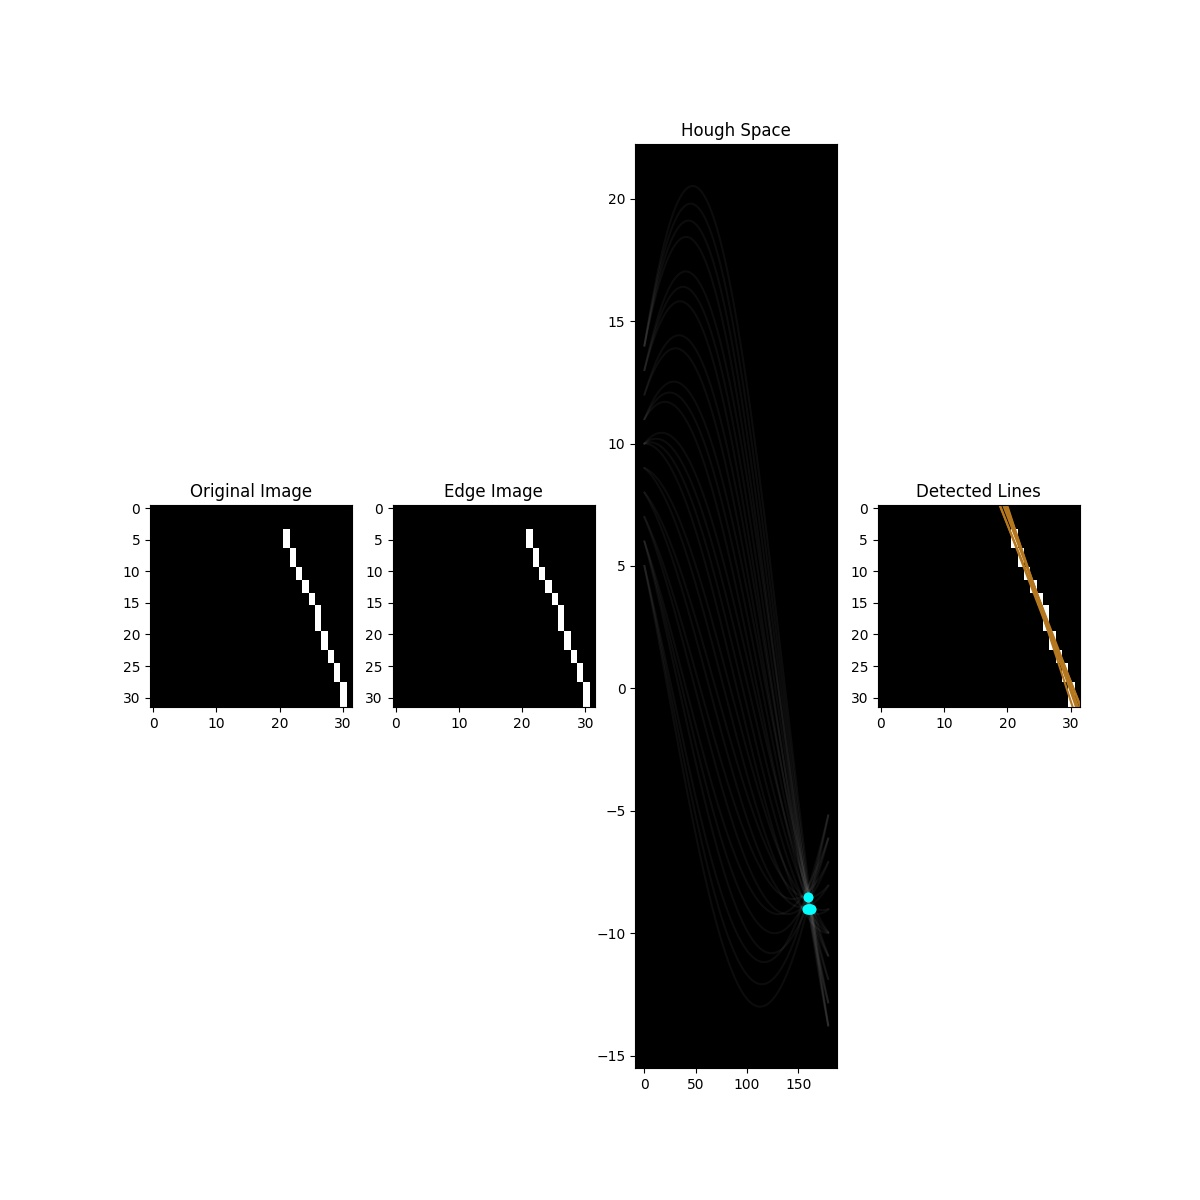
\includegraphics[width=0.6\linewidth, height=6cm]{images/hough_validation.jpg} 
        \caption{Validating Hough Transform and visualizing the detected lane segment from a single tile}
        % \caption{}
        % \label{fig:subim2}
        % \end{subfigure}
        \end{figure}
\end{frame}

\begin{frame}{Validating Hough Transform (2/2)}
% \begin{figure}
%    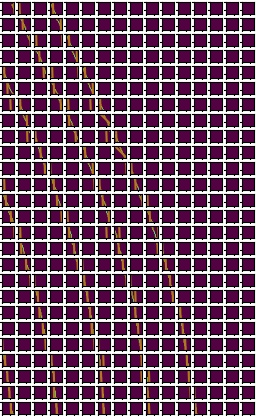
\includegraphics[scale=0.2]{images/detected_lines_r.jpg}
%    \hfill
%    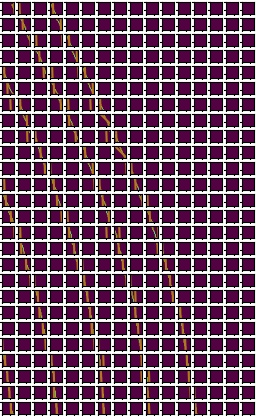
\includegraphics[scale=0.2]{images/detected_lines_r.jpg}
   
% \end{figure}    

\begin{figure}

    \caption{(Left) Detected lanes via Hough Transform, (Right) Detected lanes via Hough Transform and using Hesse normal form as a post-processing step }
   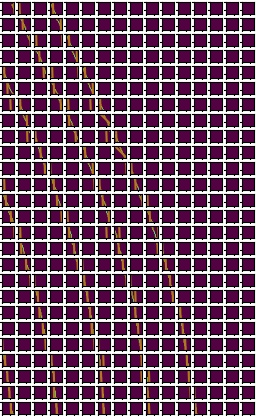
\includegraphics[width=0.3\textwidth, height=5cm]{images/detected_lines_r.jpg}
   \hfill
   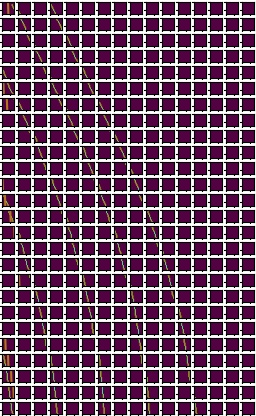
\includegraphics[width=0.3\textwidth,height=5cm]{images/detected_lines_rprime.jpg}
\end{figure}

\end{frame}



\begin{frame}{Future Work}

\begin{itemize}

    \item Solve the issue of representation of geometric 3D lane parameters.
    \item Enable the approach to generalize well with different cameras.
    \item Train the proposed approach with large-scale real-world datasets like OpenLane\footcite{chen2022persformer}.
    \item Extend this approach towards an end-to-end driving policy, where 3D lane detection will be used as an auxiliary task.
    \item Add more relatable auxiliary tasks like depth estimation, object detection.
    \item Choose appropriate task loss balancing strategy.  



\end{itemize}
    
\end{frame}


\end{document}
